% Chapter 2: Classical distributions and stylised facts
% Statistics of Financial Markets -- Bachelor's programme, Bucharest University of Economic Studies
% GENERATED by latex/build_chapter2.py -- edit the generator, not this file.

\newcommand{\coursename}{Statistics of Financial Markets}
% Preambul comun SFM -- Statistica piețelor financiare / Statistics of Financial Markets (Beamer, 16:9)
% Același design ca MFM. Înainte de % Preambul comun SFM -- Statistica piețelor financiare / Statistics of Financial Markets (Beamer, 16:9)
% Același design ca MFM. Înainte de % Preambul comun SFM -- Statistica piețelor financiare / Statistics of Financial Markets (Beamer, 16:9)
% Același design ca MFM. Înainte de \input{../../latex/preamble} se definește
%   \newcommand{\coursename}{Statistics of Financial Markets}      (EN)
%   \newcommand{\coursename}{Statistica piețelor financiare}       (RO)  și  \def\sfmlang{ro}
% Fișierele .tex se află în EN/Courses, EN/Seminars, RO/Cursuri, RO/Seminarii (două niveluri sub rădăcină).
% Deck-urile sînt generate de latex/build_chapterN.py / build_seminarN.py (vezi latex/sfm_build.py).

\documentclass[9pt, aspectratio=169, t]{beamer}
\providecommand{\coursename}{Statistics of Financial Markets}

% Ensure content fits on slides
\setbeamersize{text margin left=8mm, text margin right=8mm}

%=============================================================================
% THEME AND STYLE CONFIGURATION
%=============================================================================
\usetheme{default}
% Using default theme for clean header/footer control

% Color Palette (matching Redispatch PDF)
\definecolor{MainBlue}{RGB}{26, 58, 110}
\definecolor{AccentBlue}{RGB}{26, 58, 110}
\definecolor{IDAred}{RGB}{205, 0, 0}
\definecolor{DarkGray}{RGB}{51, 51, 51}
\definecolor{MediumGray}{RGB}{128, 128, 128}
\definecolor{LightGray}{RGB}{248, 248, 248}
\definecolor{VeryLightGray}{RGB}{235, 235, 235}
\definecolor{KeynoteGray}{RGB}{218, 218, 218}
\definecolor{SectionGray}{RGB}{120, 120, 120}
\definecolor{FooterGray}{RGB}{100, 100, 100}
\definecolor{Crimson}{RGB}{220, 53, 69}
\definecolor{Forest}{RGB}{46, 125, 50}
\definecolor{Amber}{RGB}{181, 133, 63}
\definecolor{Orange}{RGB}{230, 126, 34}
\definecolor{Purple}{RGB}{142, 68, 173}

% Gradient background (exact Keynote 315° gradient: white to RGB 218,218,218)
\setbeamertemplate{background}{%
    \begin{tikzpicture}[remember picture, overlay]
        \shade[shading=axis, shading angle=315,
        top color=white, bottom color=KeynoteGray]
        (current page.south west) rectangle (current page.north east);
    \end{tikzpicture}%
}
% Fallback solid color for compatibility
\setbeamercolor{background canvas}{bg=}

\setbeamercolor{palette primary}{bg=MainBlue, fg=white}
\setbeamercolor{palette secondary}{bg=MainBlue!85, fg=white}
\setbeamercolor{palette tertiary}{bg=MainBlue!70, fg=white}
\setbeamercolor{structure}{fg=MainBlue}
\setbeamercolor{title}{fg=IDAred}
\setbeamercolor{frametitle}{fg=IDAred, bg=}
\setbeamercolor{block title}{bg=MainBlue, fg=white}
\setbeamercolor{block body}{bg=VeryLightGray, fg=DarkGray}
\setbeamercolor{block title alerted}{bg=Crimson, fg=white}
\setbeamercolor{block body alerted}{bg=Crimson!8, fg=DarkGray}
\setbeamercolor{block title example}{bg=Forest, fg=white}
\setbeamercolor{block body example}{bg=Forest!8, fg=DarkGray}
\setbeamercolor{item}{fg=MainBlue}

% Footer colors (override Madrid theme blue)
\setbeamercolor{author in head/foot}{fg=FooterGray, bg=}
\setbeamercolor{title in head/foot}{fg=FooterGray, bg=}
\setbeamercolor{date in head/foot}{fg=FooterGray, bg=}
\setbeamercolor{section in head/foot}{fg=FooterGray, bg=}
\setbeamercolor{subsection in head/foot}{fg=FooterGray, bg=}

% Bullet styles (apply everywhere including blocks)
\setbeamertemplate{itemize item}{\color{MainBlue}$\boxdot$}
\setbeamertemplate{itemize subitem}{\color{MainBlue}$\blacktriangleright$}
\setbeamertemplate{itemize subsubitem}{\color{MainBlue}\tiny$\bullet$}
\setbeamertemplate{itemize/enumerate body begin}{\normalsize}
\setbeamertemplate{itemize/enumerate subbody begin}{\normalsize}

% Item spacing - compact style
\setlength{\leftmargini}{10pt}       % Level 1: minimal indent
\setlength{\leftmarginii}{10pt}      % Level 2: minimal additional indent
% Compact list spacing (zero extra space before/after lists in blocks)
\makeatletter
\def\@listi{\leftmargin\leftmargini \topsep 0pt \parsep 0pt \itemsep 0pt}
\def\@listii{\leftmargin\leftmarginii \topsep 0pt \parsep 0pt \itemsep 0pt}
\makeatother

\setbeamertemplate{navigation symbols}{}

%=============================================================================
% CUSTOM HEADLINE
%=============================================================================
\setbeamertemplate{headline}{%
    \vskip10pt%
    \hbox to \paperwidth{%
        \hskip0.5cm%
        {\small\color{FooterGray}\renewcommand{\hyperlink}[2]{##2}\insertsectionhead}%
        \hfill%
        \textcolor{FooterGray}{\small\insertframenumber}%
        \hskip0.5cm%
    }%
    \vskip4pt%
    {\color{FooterGray}\hrule height 0.4pt}%
}

%=============================================================================
% CUSTOM FOOTER
%=============================================================================
\usepackage{fontawesome5}

\setbeamertemplate{footline}{%
    {\color{FooterGray}\hrule height 0.4pt}%
    \vskip4pt%
    \hbox to \paperwidth{%
        \hskip0.5cm%
        \textcolor{FooterGray}{\small\coursename}%
        \hfill%
        \raisebox{-0.1em}{%
            \begin{tikzpicture}[x=0.08em, y=0.08em, line width=0.4pt]
                \draw[FooterGray] (0,3) -- (1,4) -- (2,3.5) -- (3,5) -- (4,4) -- (5,6) -- (6,5.5) -- (7,4) -- (8,5) -- (9,7) -- (10,6) -- (11,5) -- (12,6.5) -- (13,8) -- (14,7) -- (15,6) -- (16,7.5) -- (17,9) -- (18,8) -- (19,7) -- (20,8.5) -- (21,10) -- (22,9) -- (23,8) -- (24,9.5);
            \end{tikzpicture}%
        }%
        \hskip0.5cm%
    }%
    \vskip6pt%
}

%=============================================================================
% PACKAGES
%=============================================================================
\usepackage[utf8]{inputenc}
\DeclareUnicodeCharacter{03B1}{\ensuremath{\alpha}}
\usepackage[T1]{fontenc}
\usepackage{amsmath, amssymb, amsthm}
\usepackage{mathtools}
\usepackage{bm}
\usepackage{tikz}
\usetikzlibrary{arrows.meta, positioning, shapes, calc, decorations.pathreplacing, shadings}
\usepackage{booktabs}
\usepackage{multirow}
\usepackage{array}
\usepackage{graphicx}
\usepackage{hyperref}
\usepackage{colortbl}
\usepackage{listings}
\lstset{language=Python, basicstyle=\ttfamily\scriptsize, keywordstyle=\color{MainBlue}\bfseries,
  commentstyle=\color{Forest}, stringstyle=\color{Crimson}, breaklines=true,
  frame=none, backgroundcolor=\color{VeryLightGray}, xleftmargin=2mm}
\hypersetup{colorlinks=true, linkcolor=MainBlue, urlcolor=MainBlue}
\graphicspath{{../../logos/}{../../charts/}{../../photos/}}
\usepackage{xcolor}
\hfuzz=2pt  % Suppress tiny overfull warnings (<2pt)
\vfuzz=2pt  % Suppress tiny vertical overfull warnings (<2pt)

%=============================================================================
% QUANTLET COMMANDS
%   \quantlet{<displayed name>}{<url>}       (generic, compatible with the older SFM decks)
%   \sfmquantlet{Ch_05}{SFM_ch5_garch}       -> https://github.com/danpele/SFM/tree/main/Quantlets/Ch_05/SFM_ch5_garch
%   \qlurl{<folder>} is defined per chapter by the generator (Quantlets/Ch_NN/<folder>)
%=============================================================================
\newcommand{\sfmrepo}{https://github.com/danpele/SFM}
\newcommand{\sfmqlbase}{https://github.com/danpele/SFM/tree/main/Quantlets}
\newcommand{\quantlet}[2]{%
    \hfill\href{#2}{%
        \raisebox{-0.15em}{
\includegraphics[height=0.7em]{ql_logo.png}}%
        \textcolor{MainBlue}{\tiny\ #1}%
    }%
}
\newcommand{\sfmquantlet}[2]{\quantlet{\detokenize{#2}}{\sfmqlbase/#1/#2}}

%=============================================================================
% NOTEBOOKS (Google Colab)
%   \colaburl{notebooks/EN/chapter5_seminar_notebook.ipynb} -> the Colab link of a file in the SFM repo
%   \nb: the chapter notebook (each seminar deck redefines it with \renewcommand)
%=============================================================================
\newcommand{\colaburl}[1]{https://colab.research.google.com/github/danpele/SFM/blob/main/#1}
\newcommand{\nb}{https://colab.research.google.com/github/danpele/SFM/tree/main/notebooks/EN}
\newcommand{\nbname}{notebooks/EN}

%=============================================================================
% SLIDE HELPERS (used by the generators; the same as in MFM)
%=============================================================================
% local font size for list bodies (the preamble forces \normalsize)
\newcommand{\itemsize}[1]{\setbeamertemplate{itemize/enumerate body begin}{#1}\setbeamertemplate{itemize/enumerate subbody begin}{#1}}
\newcommand{\intitle}[1]{{\hypersetup{urlcolor=white}#1}}   % white links inside coloured title bars
\newcommand{\imgcap}[1]{{\scriptsize #1}\\[0.5mm]}          % caption under a photo
\newcommand{\imgcredit}[2]{{\tiny\color{FooterGray}\href{#1}{#2}}}   % image credit: source URL, author/licence
\newcommand{\aiprompt}[1]{{\ttfamily\color{MainBlue}#1}}     % a prompt to an AI assistant

%=============================================================================
% SEMINARS: student version by default; the instructor wrapper *_solutions.tex sets \solutionstrue
%=============================================================================
\makeatletter\@ifundefined{ifsolutions}{\expandafter\newif\csname ifsolutions\endcsname}{}\makeatother
\newcommand{\solonly}[1]{\ifsolutions #1\fi}
\newcommand{\propsub}{\ifsolutions\else\framesubtitle{\ifdefined\sfmlang Rezolvarea se discută la seminar\else Solution discussed in class\fi}\fi}

%=============================================================================
% APPENDIX AND CHAPTER LINKS (latex/appendix_links.py writes the calls; it also re-declares these
% macros before \begin{document}, so the decks compile with or without this preamble block)
%=============================================================================
\providecommand{\sfmapplink}[3]{\hypertarget{#2}{}\hyperlink{#1}{\beamergotobutton{#3}}}
\providecommand{\sfmappback}[2]{\begin{tikzpicture}[remember picture,overlay]\node[anchor=south east] at ([xshift=-3mm,yshift=7mm]current page.south east){\hyperlink{#1}{\beamerreturnbutton{#2}}};\end{tikzpicture}}
\providecommand{\sfmchlink}[2]{\href{#1}{#2}}
\providecommand{\sfmchlinkt}[2]{\href{#1}{\usebeamercolor[fg]{frametitle}#2}}

%=============================================================================
% QUANTINAR COMMAND: link către un curs Quantinar (subiecte avansate)
%=============================================================================
\newcommand{\quantinar}[2]{%
    \href{#2}{%
        \raisebox{-0.15em}{
\includegraphics[height=0.8em]{qr_logo.png}}%
        \textcolor{MainBlue}{\scriptsize\ #1}%
    }%
}

%=============================================================================
% CUSTOM TITLE PAGE
%=============================================================================
\defbeamertemplate*{title page}{hybrid}[1][]
{
    \vspace{0.2cm}
    % Logos row - top header (with clickable links)
    \begin{center}
        \href{https://www.ase.ro}{
\includegraphics[height=1.0cm]{ase_logo.png}}\hspace{0.3cm}%
        \href{https://theida.net}{
\includegraphics[height=1.0cm]{ida_logo.png}}\hspace{0.3cm}%
        \href{https://blockchain-research-center.com}{
\includegraphics[height=1.0cm]{brc_logo.png}}\hspace{0.3cm}%
        \href{https://www.ai4efin.ase.ro}{
\includegraphics[height=1.0cm]{ai4efin_logo.png}}\hspace{0.3cm}%
        \href{https://ipe.ro/new}{
\includegraphics[height=1.0cm]{acad_logo.png}}\hspace{0.3cm}%
        \href{https://www.digital-finance-msca.com}{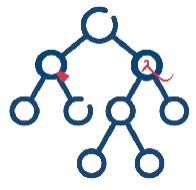
\includegraphics[height=1.0cm]{msca_logo.png}}%
    \end{center}

    \vspace{0.6cm}

    % Main title with Q logos on sides (with clickable links)
    \begin{center}
        \begin{minipage}{0.1\textwidth}
            \centering
            \href{https://quantlet.com}{
\includegraphics[height=1.1cm]{ql_logo.png}}
        \end{minipage}%
        \begin{minipage}{0.78\textwidth}
            \centering
            {\LARGE\bfseries\usebeamercolor[fg]{title}\inserttitle}

            \vspace{0.3cm}

            {\usebeamerfont{subtitle}\usebeamercolor[fg]{title}\insertsubtitle}
        \end{minipage}%
        \begin{minipage}{0.1\textwidth}
            \centering
            \href{https://quantinar.com}{
\includegraphics[height=1.1cm]{qr_logo.png}}
        \end{minipage}
    \end{center}

    \vspace{0.6cm}

    % Authors (left aligned)
    \hspace{0.5cm}{\usebeamerfont{author}\insertauthor}

    \vspace{0.3cm}

    % Institute/Affiliations (left aligned)
    \hspace{0.5cm}\begin{minipage}[t]{0.9\textwidth}
        \raggedright\small\insertinstitute
    \end{minipage}
}

%=============================================================================
% THEOREM ENVIRONMENTS
%=============================================================================
\theoremstyle{definition}
\setbeamertemplate{theorems}[numbered]
\ifdefined\sfmlang
\newtheorem{defn}{Definiție}
\newtheorem{thm}{Teoremă}
\newtheorem{prop}{Propoziție}
\newtheorem{rmk}{Observație}
\else
\newtheorem{defn}{Definition}
\newtheorem{thm}{Theorem}
\newtheorem{prop}{Proposition}
\newtheorem{rmk}{Remark}
\fi

%=============================================================================
% CENTRED MINIPAGE (no extra vertical space)
%=============================================================================
\newenvironment{cminipage}[1]{%
    \par\noindent\hfill\begin{minipage}{#1}\ignorespaces
}{%
    \end{minipage}\hfill\null\par
}

%=============================================================================
% CUSTOM COMMANDS
%=============================================================================
\newcommand{\E}{\mathbb{E}}
\newcommand{\Var}{\text{Var}}
\newcommand{\Cov}{\text{Cov}}
\newcommand{\Corr}{\text{Corr}}
\newcommand{\R}{\mathbb{R}}
\newcommand{\N}{\mathbb{N}}
\newcommand{\Z}{\mathbb{Z}}
\newcommand{\B}{\mathbf{B}}
\newcommand{\imark}{\textcolor{MainBlue}{\textbullet}}
\newcommand{\RMSE}{\text{RMSE}}
\newcommand{\MAE}{\text{MAE}}
\newcommand{\MAPE}{\text{MAPE}}

 se definește
%   \newcommand{\coursename}{Statistics of Financial Markets}      (EN)
%   \newcommand{\coursename}{Statistica piețelor financiare}       (RO)  și  \def\sfmlang{ro}
% Fișierele .tex se află în EN/Courses, EN/Seminars, RO/Cursuri, RO/Seminarii (două niveluri sub rădăcină).
% Deck-urile sînt generate de latex/build_chapterN.py / build_seminarN.py (vezi latex/sfm_build.py).

\documentclass[9pt, aspectratio=169, t]{beamer}
\providecommand{\coursename}{Statistics of Financial Markets}

% Ensure content fits on slides
\setbeamersize{text margin left=8mm, text margin right=8mm}

%=============================================================================
% THEME AND STYLE CONFIGURATION
%=============================================================================
\usetheme{default}
% Using default theme for clean header/footer control

% Color Palette (matching Redispatch PDF)
\definecolor{MainBlue}{RGB}{26, 58, 110}
\definecolor{AccentBlue}{RGB}{26, 58, 110}
\definecolor{IDAred}{RGB}{205, 0, 0}
\definecolor{DarkGray}{RGB}{51, 51, 51}
\definecolor{MediumGray}{RGB}{128, 128, 128}
\definecolor{LightGray}{RGB}{248, 248, 248}
\definecolor{VeryLightGray}{RGB}{235, 235, 235}
\definecolor{KeynoteGray}{RGB}{218, 218, 218}
\definecolor{SectionGray}{RGB}{120, 120, 120}
\definecolor{FooterGray}{RGB}{100, 100, 100}
\definecolor{Crimson}{RGB}{220, 53, 69}
\definecolor{Forest}{RGB}{46, 125, 50}
\definecolor{Amber}{RGB}{181, 133, 63}
\definecolor{Orange}{RGB}{230, 126, 34}
\definecolor{Purple}{RGB}{142, 68, 173}

% Gradient background (exact Keynote 315° gradient: white to RGB 218,218,218)
\setbeamertemplate{background}{%
    \begin{tikzpicture}[remember picture, overlay]
        \shade[shading=axis, shading angle=315,
        top color=white, bottom color=KeynoteGray]
        (current page.south west) rectangle (current page.north east);
    \end{tikzpicture}%
}
% Fallback solid color for compatibility
\setbeamercolor{background canvas}{bg=}

\setbeamercolor{palette primary}{bg=MainBlue, fg=white}
\setbeamercolor{palette secondary}{bg=MainBlue!85, fg=white}
\setbeamercolor{palette tertiary}{bg=MainBlue!70, fg=white}
\setbeamercolor{structure}{fg=MainBlue}
\setbeamercolor{title}{fg=IDAred}
\setbeamercolor{frametitle}{fg=IDAred, bg=}
\setbeamercolor{block title}{bg=MainBlue, fg=white}
\setbeamercolor{block body}{bg=VeryLightGray, fg=DarkGray}
\setbeamercolor{block title alerted}{bg=Crimson, fg=white}
\setbeamercolor{block body alerted}{bg=Crimson!8, fg=DarkGray}
\setbeamercolor{block title example}{bg=Forest, fg=white}
\setbeamercolor{block body example}{bg=Forest!8, fg=DarkGray}
\setbeamercolor{item}{fg=MainBlue}

% Footer colors (override Madrid theme blue)
\setbeamercolor{author in head/foot}{fg=FooterGray, bg=}
\setbeamercolor{title in head/foot}{fg=FooterGray, bg=}
\setbeamercolor{date in head/foot}{fg=FooterGray, bg=}
\setbeamercolor{section in head/foot}{fg=FooterGray, bg=}
\setbeamercolor{subsection in head/foot}{fg=FooterGray, bg=}

% Bullet styles (apply everywhere including blocks)
\setbeamertemplate{itemize item}{\color{MainBlue}$\boxdot$}
\setbeamertemplate{itemize subitem}{\color{MainBlue}$\blacktriangleright$}
\setbeamertemplate{itemize subsubitem}{\color{MainBlue}\tiny$\bullet$}
\setbeamertemplate{itemize/enumerate body begin}{\normalsize}
\setbeamertemplate{itemize/enumerate subbody begin}{\normalsize}

% Item spacing - compact style
\setlength{\leftmargini}{10pt}       % Level 1: minimal indent
\setlength{\leftmarginii}{10pt}      % Level 2: minimal additional indent
% Compact list spacing (zero extra space before/after lists in blocks)
\makeatletter
\def\@listi{\leftmargin\leftmargini \topsep 0pt \parsep 0pt \itemsep 0pt}
\def\@listii{\leftmargin\leftmarginii \topsep 0pt \parsep 0pt \itemsep 0pt}
\makeatother

\setbeamertemplate{navigation symbols}{}

%=============================================================================
% CUSTOM HEADLINE
%=============================================================================
\setbeamertemplate{headline}{%
    \vskip10pt%
    \hbox to \paperwidth{%
        \hskip0.5cm%
        {\small\color{FooterGray}\renewcommand{\hyperlink}[2]{##2}\insertsectionhead}%
        \hfill%
        \textcolor{FooterGray}{\small\insertframenumber}%
        \hskip0.5cm%
    }%
    \vskip4pt%
    {\color{FooterGray}\hrule height 0.4pt}%
}

%=============================================================================
% CUSTOM FOOTER
%=============================================================================
\usepackage{fontawesome5}

\setbeamertemplate{footline}{%
    {\color{FooterGray}\hrule height 0.4pt}%
    \vskip4pt%
    \hbox to \paperwidth{%
        \hskip0.5cm%
        \textcolor{FooterGray}{\small\coursename}%
        \hfill%
        \raisebox{-0.1em}{%
            \begin{tikzpicture}[x=0.08em, y=0.08em, line width=0.4pt]
                \draw[FooterGray] (0,3) -- (1,4) -- (2,3.5) -- (3,5) -- (4,4) -- (5,6) -- (6,5.5) -- (7,4) -- (8,5) -- (9,7) -- (10,6) -- (11,5) -- (12,6.5) -- (13,8) -- (14,7) -- (15,6) -- (16,7.5) -- (17,9) -- (18,8) -- (19,7) -- (20,8.5) -- (21,10) -- (22,9) -- (23,8) -- (24,9.5);
            \end{tikzpicture}%
        }%
        \hskip0.5cm%
    }%
    \vskip6pt%
}

%=============================================================================
% PACKAGES
%=============================================================================
\usepackage[utf8]{inputenc}
\DeclareUnicodeCharacter{03B1}{\ensuremath{\alpha}}
\usepackage[T1]{fontenc}
\usepackage{amsmath, amssymb, amsthm}
\usepackage{mathtools}
\usepackage{bm}
\usepackage{tikz}
\usetikzlibrary{arrows.meta, positioning, shapes, calc, decorations.pathreplacing, shadings}
\usepackage{booktabs}
\usepackage{multirow}
\usepackage{array}
\usepackage{graphicx}
\usepackage{hyperref}
\usepackage{colortbl}
\usepackage{listings}
\lstset{language=Python, basicstyle=\ttfamily\scriptsize, keywordstyle=\color{MainBlue}\bfseries,
  commentstyle=\color{Forest}, stringstyle=\color{Crimson}, breaklines=true,
  frame=none, backgroundcolor=\color{VeryLightGray}, xleftmargin=2mm}
\hypersetup{colorlinks=true, linkcolor=MainBlue, urlcolor=MainBlue}
\graphicspath{{../../logos/}{../../charts/}{../../photos/}}
\usepackage{xcolor}
\hfuzz=2pt  % Suppress tiny overfull warnings (<2pt)
\vfuzz=2pt  % Suppress tiny vertical overfull warnings (<2pt)

%=============================================================================
% QUANTLET COMMANDS
%   \quantlet{<displayed name>}{<url>}       (generic, compatible with the older SFM decks)
%   \sfmquantlet{Ch_05}{SFM_ch5_garch}       -> https://github.com/danpele/SFM/tree/main/Quantlets/Ch_05/SFM_ch5_garch
%   \qlurl{<folder>} is defined per chapter by the generator (Quantlets/Ch_NN/<folder>)
%=============================================================================
\newcommand{\sfmrepo}{https://github.com/danpele/SFM}
\newcommand{\sfmqlbase}{https://github.com/danpele/SFM/tree/main/Quantlets}
\newcommand{\quantlet}[2]{%
    \hfill\href{#2}{%
        \raisebox{-0.15em}{
\includegraphics[height=0.7em]{ql_logo.png}}%
        \textcolor{MainBlue}{\tiny\ #1}%
    }%
}
\newcommand{\sfmquantlet}[2]{\quantlet{\detokenize{#2}}{\sfmqlbase/#1/#2}}

%=============================================================================
% NOTEBOOKS (Google Colab)
%   \colaburl{notebooks/EN/chapter5_seminar_notebook.ipynb} -> the Colab link of a file in the SFM repo
%   \nb: the chapter notebook (each seminar deck redefines it with \renewcommand)
%=============================================================================
\newcommand{\colaburl}[1]{https://colab.research.google.com/github/danpele/SFM/blob/main/#1}
\newcommand{\nb}{https://colab.research.google.com/github/danpele/SFM/tree/main/notebooks/EN}
\newcommand{\nbname}{notebooks/EN}

%=============================================================================
% SLIDE HELPERS (used by the generators; the same as in MFM)
%=============================================================================
% local font size for list bodies (the preamble forces \normalsize)
\newcommand{\itemsize}[1]{\setbeamertemplate{itemize/enumerate body begin}{#1}\setbeamertemplate{itemize/enumerate subbody begin}{#1}}
\newcommand{\intitle}[1]{{\hypersetup{urlcolor=white}#1}}   % white links inside coloured title bars
\newcommand{\imgcap}[1]{{\scriptsize #1}\\[0.5mm]}          % caption under a photo
\newcommand{\imgcredit}[2]{{\tiny\color{FooterGray}\href{#1}{#2}}}   % image credit: source URL, author/licence
\newcommand{\aiprompt}[1]{{\ttfamily\color{MainBlue}#1}}     % a prompt to an AI assistant

%=============================================================================
% SEMINARS: student version by default; the instructor wrapper *_solutions.tex sets \solutionstrue
%=============================================================================
\makeatletter\@ifundefined{ifsolutions}{\expandafter\newif\csname ifsolutions\endcsname}{}\makeatother
\newcommand{\solonly}[1]{\ifsolutions #1\fi}
\newcommand{\propsub}{\ifsolutions\else\framesubtitle{\ifdefined\sfmlang Rezolvarea se discută la seminar\else Solution discussed in class\fi}\fi}

%=============================================================================
% APPENDIX AND CHAPTER LINKS (latex/appendix_links.py writes the calls; it also re-declares these
% macros before \begin{document}, so the decks compile with or without this preamble block)
%=============================================================================
\providecommand{\sfmapplink}[3]{\hypertarget{#2}{}\hyperlink{#1}{\beamergotobutton{#3}}}
\providecommand{\sfmappback}[2]{\begin{tikzpicture}[remember picture,overlay]\node[anchor=south east] at ([xshift=-3mm,yshift=7mm]current page.south east){\hyperlink{#1}{\beamerreturnbutton{#2}}};\end{tikzpicture}}
\providecommand{\sfmchlink}[2]{\href{#1}{#2}}
\providecommand{\sfmchlinkt}[2]{\href{#1}{\usebeamercolor[fg]{frametitle}#2}}

%=============================================================================
% QUANTINAR COMMAND: link către un curs Quantinar (subiecte avansate)
%=============================================================================
\newcommand{\quantinar}[2]{%
    \href{#2}{%
        \raisebox{-0.15em}{
\includegraphics[height=0.8em]{qr_logo.png}}%
        \textcolor{MainBlue}{\scriptsize\ #1}%
    }%
}

%=============================================================================
% CUSTOM TITLE PAGE
%=============================================================================
\defbeamertemplate*{title page}{hybrid}[1][]
{
    \vspace{0.2cm}
    % Logos row - top header (with clickable links)
    \begin{center}
        \href{https://www.ase.ro}{
\includegraphics[height=1.0cm]{ase_logo.png}}\hspace{0.3cm}%
        \href{https://theida.net}{
\includegraphics[height=1.0cm]{ida_logo.png}}\hspace{0.3cm}%
        \href{https://blockchain-research-center.com}{
\includegraphics[height=1.0cm]{brc_logo.png}}\hspace{0.3cm}%
        \href{https://www.ai4efin.ase.ro}{
\includegraphics[height=1.0cm]{ai4efin_logo.png}}\hspace{0.3cm}%
        \href{https://ipe.ro/new}{
\includegraphics[height=1.0cm]{acad_logo.png}}\hspace{0.3cm}%
        \href{https://www.digital-finance-msca.com}{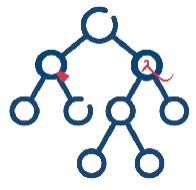
\includegraphics[height=1.0cm]{msca_logo.png}}%
    \end{center}

    \vspace{0.6cm}

    % Main title with Q logos on sides (with clickable links)
    \begin{center}
        \begin{minipage}{0.1\textwidth}
            \centering
            \href{https://quantlet.com}{
\includegraphics[height=1.1cm]{ql_logo.png}}
        \end{minipage}%
        \begin{minipage}{0.78\textwidth}
            \centering
            {\LARGE\bfseries\usebeamercolor[fg]{title}\inserttitle}

            \vspace{0.3cm}

            {\usebeamerfont{subtitle}\usebeamercolor[fg]{title}\insertsubtitle}
        \end{minipage}%
        \begin{minipage}{0.1\textwidth}
            \centering
            \href{https://quantinar.com}{
\includegraphics[height=1.1cm]{qr_logo.png}}
        \end{minipage}
    \end{center}

    \vspace{0.6cm}

    % Authors (left aligned)
    \hspace{0.5cm}{\usebeamerfont{author}\insertauthor}

    \vspace{0.3cm}

    % Institute/Affiliations (left aligned)
    \hspace{0.5cm}\begin{minipage}[t]{0.9\textwidth}
        \raggedright\small\insertinstitute
    \end{minipage}
}

%=============================================================================
% THEOREM ENVIRONMENTS
%=============================================================================
\theoremstyle{definition}
\setbeamertemplate{theorems}[numbered]
\ifdefined\sfmlang
\newtheorem{defn}{Definiție}
\newtheorem{thm}{Teoremă}
\newtheorem{prop}{Propoziție}
\newtheorem{rmk}{Observație}
\else
\newtheorem{defn}{Definition}
\newtheorem{thm}{Theorem}
\newtheorem{prop}{Proposition}
\newtheorem{rmk}{Remark}
\fi

%=============================================================================
% CENTRED MINIPAGE (no extra vertical space)
%=============================================================================
\newenvironment{cminipage}[1]{%
    \par\noindent\hfill\begin{minipage}{#1}\ignorespaces
}{%
    \end{minipage}\hfill\null\par
}

%=============================================================================
% CUSTOM COMMANDS
%=============================================================================
\newcommand{\E}{\mathbb{E}}
\newcommand{\Var}{\text{Var}}
\newcommand{\Cov}{\text{Cov}}
\newcommand{\Corr}{\text{Corr}}
\newcommand{\R}{\mathbb{R}}
\newcommand{\N}{\mathbb{N}}
\newcommand{\Z}{\mathbb{Z}}
\newcommand{\B}{\mathbf{B}}
\newcommand{\imark}{\textcolor{MainBlue}{\textbullet}}
\newcommand{\RMSE}{\text{RMSE}}
\newcommand{\MAE}{\text{MAE}}
\newcommand{\MAPE}{\text{MAPE}}

 se definește
%   \newcommand{\coursename}{Statistics of Financial Markets}      (EN)
%   \newcommand{\coursename}{Statistica piețelor financiare}       (RO)  și  \def\sfmlang{ro}
% Fișierele .tex se află în EN/Courses, EN/Seminars, RO/Cursuri, RO/Seminarii (două niveluri sub rădăcină).
% Deck-urile sînt generate de latex/build_chapterN.py / build_seminarN.py (vezi latex/sfm_build.py).

\documentclass[9pt, aspectratio=169, t]{beamer}
\providecommand{\coursename}{Statistics of Financial Markets}

% Ensure content fits on slides
\setbeamersize{text margin left=8mm, text margin right=8mm}

%=============================================================================
% THEME AND STYLE CONFIGURATION
%=============================================================================
\usetheme{default}
% Using default theme for clean header/footer control

% Color Palette (matching Redispatch PDF)
\definecolor{MainBlue}{RGB}{26, 58, 110}
\definecolor{AccentBlue}{RGB}{26, 58, 110}
\definecolor{IDAred}{RGB}{205, 0, 0}
\definecolor{DarkGray}{RGB}{51, 51, 51}
\definecolor{MediumGray}{RGB}{128, 128, 128}
\definecolor{LightGray}{RGB}{248, 248, 248}
\definecolor{VeryLightGray}{RGB}{235, 235, 235}
\definecolor{KeynoteGray}{RGB}{218, 218, 218}
\definecolor{SectionGray}{RGB}{120, 120, 120}
\definecolor{FooterGray}{RGB}{100, 100, 100}
\definecolor{Crimson}{RGB}{220, 53, 69}
\definecolor{Forest}{RGB}{46, 125, 50}
\definecolor{Amber}{RGB}{181, 133, 63}
\definecolor{Orange}{RGB}{230, 126, 34}
\definecolor{Purple}{RGB}{142, 68, 173}

% Gradient background (exact Keynote 315° gradient: white to RGB 218,218,218)
\setbeamertemplate{background}{%
    \begin{tikzpicture}[remember picture, overlay]
        \shade[shading=axis, shading angle=315,
        top color=white, bottom color=KeynoteGray]
        (current page.south west) rectangle (current page.north east);
    \end{tikzpicture}%
}
% Fallback solid color for compatibility
\setbeamercolor{background canvas}{bg=}

\setbeamercolor{palette primary}{bg=MainBlue, fg=white}
\setbeamercolor{palette secondary}{bg=MainBlue!85, fg=white}
\setbeamercolor{palette tertiary}{bg=MainBlue!70, fg=white}
\setbeamercolor{structure}{fg=MainBlue}
\setbeamercolor{title}{fg=IDAred}
\setbeamercolor{frametitle}{fg=IDAred, bg=}
\setbeamercolor{block title}{bg=MainBlue, fg=white}
\setbeamercolor{block body}{bg=VeryLightGray, fg=DarkGray}
\setbeamercolor{block title alerted}{bg=Crimson, fg=white}
\setbeamercolor{block body alerted}{bg=Crimson!8, fg=DarkGray}
\setbeamercolor{block title example}{bg=Forest, fg=white}
\setbeamercolor{block body example}{bg=Forest!8, fg=DarkGray}
\setbeamercolor{item}{fg=MainBlue}

% Footer colors (override Madrid theme blue)
\setbeamercolor{author in head/foot}{fg=FooterGray, bg=}
\setbeamercolor{title in head/foot}{fg=FooterGray, bg=}
\setbeamercolor{date in head/foot}{fg=FooterGray, bg=}
\setbeamercolor{section in head/foot}{fg=FooterGray, bg=}
\setbeamercolor{subsection in head/foot}{fg=FooterGray, bg=}

% Bullet styles (apply everywhere including blocks)
\setbeamertemplate{itemize item}{\color{MainBlue}$\boxdot$}
\setbeamertemplate{itemize subitem}{\color{MainBlue}$\blacktriangleright$}
\setbeamertemplate{itemize subsubitem}{\color{MainBlue}\tiny$\bullet$}
\setbeamertemplate{itemize/enumerate body begin}{\normalsize}
\setbeamertemplate{itemize/enumerate subbody begin}{\normalsize}

% Item spacing - compact style
\setlength{\leftmargini}{10pt}       % Level 1: minimal indent
\setlength{\leftmarginii}{10pt}      % Level 2: minimal additional indent
% Compact list spacing (zero extra space before/after lists in blocks)
\makeatletter
\def\@listi{\leftmargin\leftmargini \topsep 0pt \parsep 0pt \itemsep 0pt}
\def\@listii{\leftmargin\leftmarginii \topsep 0pt \parsep 0pt \itemsep 0pt}
\makeatother

\setbeamertemplate{navigation symbols}{}

%=============================================================================
% CUSTOM HEADLINE
%=============================================================================
\setbeamertemplate{headline}{%
    \vskip10pt%
    \hbox to \paperwidth{%
        \hskip0.5cm%
        {\small\color{FooterGray}\renewcommand{\hyperlink}[2]{##2}\insertsectionhead}%
        \hfill%
        \textcolor{FooterGray}{\small\insertframenumber}%
        \hskip0.5cm%
    }%
    \vskip4pt%
    {\color{FooterGray}\hrule height 0.4pt}%
}

%=============================================================================
% CUSTOM FOOTER
%=============================================================================
\usepackage{fontawesome5}

\setbeamertemplate{footline}{%
    {\color{FooterGray}\hrule height 0.4pt}%
    \vskip4pt%
    \hbox to \paperwidth{%
        \hskip0.5cm%
        \textcolor{FooterGray}{\small\coursename}%
        \hfill%
        \raisebox{-0.1em}{%
            \begin{tikzpicture}[x=0.08em, y=0.08em, line width=0.4pt]
                \draw[FooterGray] (0,3) -- (1,4) -- (2,3.5) -- (3,5) -- (4,4) -- (5,6) -- (6,5.5) -- (7,4) -- (8,5) -- (9,7) -- (10,6) -- (11,5) -- (12,6.5) -- (13,8) -- (14,7) -- (15,6) -- (16,7.5) -- (17,9) -- (18,8) -- (19,7) -- (20,8.5) -- (21,10) -- (22,9) -- (23,8) -- (24,9.5);
            \end{tikzpicture}%
        }%
        \hskip0.5cm%
    }%
    \vskip6pt%
}

%=============================================================================
% PACKAGES
%=============================================================================
\usepackage[utf8]{inputenc}
\DeclareUnicodeCharacter{03B1}{\ensuremath{\alpha}}
\usepackage[T1]{fontenc}
\usepackage{amsmath, amssymb, amsthm}
\usepackage{mathtools}
\usepackage{bm}
\usepackage{tikz}
\usetikzlibrary{arrows.meta, positioning, shapes, calc, decorations.pathreplacing, shadings}
\usepackage{booktabs}
\usepackage{multirow}
\usepackage{array}
\usepackage{graphicx}
\usepackage{hyperref}
\usepackage{colortbl}
\usepackage{listings}
\lstset{language=Python, basicstyle=\ttfamily\scriptsize, keywordstyle=\color{MainBlue}\bfseries,
  commentstyle=\color{Forest}, stringstyle=\color{Crimson}, breaklines=true,
  frame=none, backgroundcolor=\color{VeryLightGray}, xleftmargin=2mm}
\hypersetup{colorlinks=true, linkcolor=MainBlue, urlcolor=MainBlue}
\graphicspath{{../../logos/}{../../charts/}{../../photos/}}
\usepackage{xcolor}
\hfuzz=2pt  % Suppress tiny overfull warnings (<2pt)
\vfuzz=2pt  % Suppress tiny vertical overfull warnings (<2pt)

%=============================================================================
% QUANTLET COMMANDS
%   \quantlet{<displayed name>}{<url>}       (generic, compatible with the older SFM decks)
%   \sfmquantlet{Ch_05}{SFM_ch5_garch}       -> https://github.com/danpele/SFM/tree/main/Quantlets/Ch_05/SFM_ch5_garch
%   \qlurl{<folder>} is defined per chapter by the generator (Quantlets/Ch_NN/<folder>)
%=============================================================================
\newcommand{\sfmrepo}{https://github.com/danpele/SFM}
\newcommand{\sfmqlbase}{https://github.com/danpele/SFM/tree/main/Quantlets}
\newcommand{\quantlet}[2]{%
    \hfill\href{#2}{%
        \raisebox{-0.15em}{
\includegraphics[height=0.7em]{ql_logo.png}}%
        \textcolor{MainBlue}{\tiny\ #1}%
    }%
}
\newcommand{\sfmquantlet}[2]{\quantlet{\detokenize{#2}}{\sfmqlbase/#1/#2}}

%=============================================================================
% NOTEBOOKS (Google Colab)
%   \colaburl{notebooks/EN/chapter5_seminar_notebook.ipynb} -> the Colab link of a file in the SFM repo
%   \nb: the chapter notebook (each seminar deck redefines it with \renewcommand)
%=============================================================================
\newcommand{\colaburl}[1]{https://colab.research.google.com/github/danpele/SFM/blob/main/#1}
\newcommand{\nb}{https://colab.research.google.com/github/danpele/SFM/tree/main/notebooks/EN}
\newcommand{\nbname}{notebooks/EN}

%=============================================================================
% SLIDE HELPERS (used by the generators; the same as in MFM)
%=============================================================================
% local font size for list bodies (the preamble forces \normalsize)
\newcommand{\itemsize}[1]{\setbeamertemplate{itemize/enumerate body begin}{#1}\setbeamertemplate{itemize/enumerate subbody begin}{#1}}
\newcommand{\intitle}[1]{{\hypersetup{urlcolor=white}#1}}   % white links inside coloured title bars
\newcommand{\imgcap}[1]{{\scriptsize #1}\\[0.5mm]}          % caption under a photo
\newcommand{\imgcredit}[2]{{\tiny\color{FooterGray}\href{#1}{#2}}}   % image credit: source URL, author/licence
\newcommand{\aiprompt}[1]{{\ttfamily\color{MainBlue}#1}}     % a prompt to an AI assistant

%=============================================================================
% SEMINARS: student version by default; the instructor wrapper *_solutions.tex sets \solutionstrue
%=============================================================================
\makeatletter\@ifundefined{ifsolutions}{\expandafter\newif\csname ifsolutions\endcsname}{}\makeatother
\newcommand{\solonly}[1]{\ifsolutions #1\fi}
\newcommand{\propsub}{\ifsolutions\else\framesubtitle{\ifdefined\sfmlang Rezolvarea se discută la seminar\else Solution discussed in class\fi}\fi}

%=============================================================================
% APPENDIX AND CHAPTER LINKS (latex/appendix_links.py writes the calls; it also re-declares these
% macros before \begin{document}, so the decks compile with or without this preamble block)
%=============================================================================
\providecommand{\sfmapplink}[3]{\hypertarget{#2}{}\hyperlink{#1}{\beamergotobutton{#3}}}
\providecommand{\sfmappback}[2]{\begin{tikzpicture}[remember picture,overlay]\node[anchor=south east] at ([xshift=-3mm,yshift=7mm]current page.south east){\hyperlink{#1}{\beamerreturnbutton{#2}}};\end{tikzpicture}}
\providecommand{\sfmchlink}[2]{\href{#1}{#2}}
\providecommand{\sfmchlinkt}[2]{\href{#1}{\usebeamercolor[fg]{frametitle}#2}}

%=============================================================================
% QUANTINAR COMMAND: link către un curs Quantinar (subiecte avansate)
%=============================================================================
\newcommand{\quantinar}[2]{%
    \href{#2}{%
        \raisebox{-0.15em}{
\includegraphics[height=0.8em]{qr_logo.png}}%
        \textcolor{MainBlue}{\scriptsize\ #1}%
    }%
}

%=============================================================================
% CUSTOM TITLE PAGE
%=============================================================================
\defbeamertemplate*{title page}{hybrid}[1][]
{
    \vspace{0.2cm}
    % Logos row - top header (with clickable links)
    \begin{center}
        \href{https://www.ase.ro}{
\includegraphics[height=1.0cm]{ase_logo.png}}\hspace{0.3cm}%
        \href{https://theida.net}{
\includegraphics[height=1.0cm]{ida_logo.png}}\hspace{0.3cm}%
        \href{https://blockchain-research-center.com}{
\includegraphics[height=1.0cm]{brc_logo.png}}\hspace{0.3cm}%
        \href{https://www.ai4efin.ase.ro}{
\includegraphics[height=1.0cm]{ai4efin_logo.png}}\hspace{0.3cm}%
        \href{https://ipe.ro/new}{
\includegraphics[height=1.0cm]{acad_logo.png}}\hspace{0.3cm}%
        \href{https://www.digital-finance-msca.com}{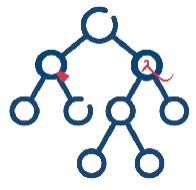
\includegraphics[height=1.0cm]{msca_logo.png}}%
    \end{center}

    \vspace{0.6cm}

    % Main title with Q logos on sides (with clickable links)
    \begin{center}
        \begin{minipage}{0.1\textwidth}
            \centering
            \href{https://quantlet.com}{
\includegraphics[height=1.1cm]{ql_logo.png}}
        \end{minipage}%
        \begin{minipage}{0.78\textwidth}
            \centering
            {\LARGE\bfseries\usebeamercolor[fg]{title}\inserttitle}

            \vspace{0.3cm}

            {\usebeamerfont{subtitle}\usebeamercolor[fg]{title}\insertsubtitle}
        \end{minipage}%
        \begin{minipage}{0.1\textwidth}
            \centering
            \href{https://quantinar.com}{
\includegraphics[height=1.1cm]{qr_logo.png}}
        \end{minipage}
    \end{center}

    \vspace{0.6cm}

    % Authors (left aligned)
    \hspace{0.5cm}{\usebeamerfont{author}\insertauthor}

    \vspace{0.3cm}

    % Institute/Affiliations (left aligned)
    \hspace{0.5cm}\begin{minipage}[t]{0.9\textwidth}
        \raggedright\small\insertinstitute
    \end{minipage}
}

%=============================================================================
% THEOREM ENVIRONMENTS
%=============================================================================
\theoremstyle{definition}
\setbeamertemplate{theorems}[numbered]
\ifdefined\sfmlang
\newtheorem{defn}{Definiție}
\newtheorem{thm}{Teoremă}
\newtheorem{prop}{Propoziție}
\newtheorem{rmk}{Observație}
\else
\newtheorem{defn}{Definition}
\newtheorem{thm}{Theorem}
\newtheorem{prop}{Proposition}
\newtheorem{rmk}{Remark}
\fi

%=============================================================================
% CENTRED MINIPAGE (no extra vertical space)
%=============================================================================
\newenvironment{cminipage}[1]{%
    \par\noindent\hfill\begin{minipage}{#1}\ignorespaces
}{%
    \end{minipage}\hfill\null\par
}

%=============================================================================
% CUSTOM COMMANDS
%=============================================================================
\newcommand{\E}{\mathbb{E}}
\newcommand{\Var}{\text{Var}}
\newcommand{\Cov}{\text{Cov}}
\newcommand{\Corr}{\text{Corr}}
\newcommand{\R}{\mathbb{R}}
\newcommand{\N}{\mathbb{N}}
\newcommand{\Z}{\mathbb{Z}}
\newcommand{\B}{\mathbf{B}}
\newcommand{\imark}{\textcolor{MainBlue}{\textbullet}}
\newcommand{\RMSE}{\text{RMSE}}
\newcommand{\MAE}{\text{MAE}}
\newcommand{\MAPE}{\text{MAPE}}



\newcommand{\qlurl}[1]{https://github.com/danpele/SFM/tree/main/Quantlets/Ch_02/#1}

% Clickable citations (DOIs verified via Crossref)

\newcommand{\refFHH}{\href{https://doi.org/10.1007/978-3-030-13751-9}{Franke, Härdle \& Hafner (2019)}}
\newcommand{\refFHHex}{\href{https://doi.org/10.1007/978-3-642-33929-5}{Borak, Härdle \& López-Cabrera (2013)}}
\newcommand{\refTsay}{\href{https://doi.org/10.1002/9780470644560}{Tsay (2010)}}
\newcommand{\refCont}{\href{https://doi.org/10.1080/713665670}{Cont (2001)}}
\newcommand{\refBachelier}{\href{https://doi.org/10.24033/asens.476}{Bachelier (1900)}}
\newcommand{\refOsborne}{\href{https://doi.org/10.1287/opre.7.2.145}{Osborne (1959)}}
\newcommand{\refMandelbrot}{\href{https://doi.org/10.1086/294632}{Mandelbrot (1963)}}
\newcommand{\refFama}{\href{https://doi.org/10.1086/294743}{Fama (1965)}}
\newcommand{\refStudent}{\href{https://doi.org/10.1093/biomet/6.1.1}{Student (1908)}}
\newcommand{\refPraetz}{\href{https://doi.org/10.1086/295425}{Praetz (1972)}}
\newcommand{\refBG}{\href{https://doi.org/10.1086/295634}{Blattberg \& Gonedes (1974)}}
\newcommand{\refJBa}{\href{https://doi.org/10.1016/0165-1765(80)90024-5}{Jarque \& Bera (1980)}}
\newcommand{\refJBb}{\href{https://doi.org/10.2307/1403192}{Jarque \& Bera (1987)}}
\newcommand{\refWG}{\href{https://doi.org/10.1093/biomet/55.1.1}{Wilk \& Gnanadesikan (1968)}}
\newcommand{\refChristie}{\href{https://doi.org/10.1016/0304-405X(82)90018-6}{Christie (1982)}}
\newcommand{\refBollerslev}{\href{https://doi.org/10.2307/1925546}{Bollerslev (1987)}}
\newcommand{\refLB}{\href{https://doi.org/10.1093/biomet/65.2.297}{Ljung \& Box (1978)}}
\newcommand{\refAkaike}{\href{https://doi.org/10.1109/TAC.1974.1100705}{Akaike (1974)}}
\newcommand{\refPeleCrypto}{\href{https://doi.org/10.1080/1351847X.2021.1960403}{Pele et al.\ (2023)}}
\newcommand{\refPeleEntropy}{\href{https://doi.org/10.3390/e19050226}{Pele, Lazar \& Dufour (2017)}}
\newcommand{\refWang}{\href{https://doi.org/10.1038/s41586-023-06221-2}{Wang et al.\ (2023)}}

\title[Statistics of Financial Markets]{Statistics of Financial Markets}
\subtitle{Chapter 2: Classical distributions and stylised facts}
\author[D.T. Pele]{Daniel Traian PELE}
\institute{Bucharest University of Economic Studies\\
IDA Institute Digital Assets\\
Blockchain Research Center\\
AI4EFin Artificial Intelligence for Energy Finance\\
Romanian Academy, Institute for Economic Forecasting\\
MSCA Digital Finance}
\date{}

%=============================================================================
\providecommand{\sfmapplink}[3]{\hypertarget{#2}{}\hyperlink{#1}{\beamergotobutton{#3}}}  % APPLINKS-MACROS
\providecommand{\sfmappback}[2]{\begin{tikzpicture}[remember picture,overlay]\node[anchor=south east] at ([xshift=-3mm,yshift=7mm]current page.south east){\hyperlink{#1}{\beamerreturnbutton{#2}}};\end{tikzpicture}}  % APPLINKS-MACROS
\providecommand{\sfmchlink}[2]{\href{#1}{#2}}  % APPLINKS-MACROS
\providecommand{\sfmchlinkt}[2]{\href{#1}{\usebeamercolor[fg]{frametitle}#2}}  % APPLINKS-MACROS
\begin{document}
%=============================================================================

{
\setbeamertemplate{headline}{}
\setbeamertemplate{footline}{}
\begin{frame}[noframenumbering]
    \titlepage
\end{frame}
}
% BEGIN-ACRONYMS (generat de latex/acronyms.py; nu editati manual)
\begin{frame}{Acronyms used in this material}
\setbeamertemplate{itemize/enumerate body begin}{\footnotesize}
\begin{columns}[T]
\begin{column}{0.49\textwidth}
\begin{itemize}\setlength{\itemsep}{0pt}
    \item \textbf{ACF}: Autocorrelation Function
    \item \textbf{AI}: Artificial Intelligence
    \item \textbf{AIC}: Akaike Information Criterion
    \item \textbf{ARCH}: AutoRegressive Conditional Heteroskedasticity
    \item \textbf{BET}: Bucharest Exchange Trading (index)
    \item \textbf{BVB}: Bursa de Valori București (the Bucharest Stock Exchange)
    \item \textbf{CDF}: Cumulative Distribution Function
    \item \textbf{CLT}: Central Limit Theorem
    \item \textbf{EGARCH}: Exponential GARCH
    \item \textbf{ES}: Expected Shortfall
\end{itemize}
\end{column}
\begin{column}{0.49\textwidth}
\begin{itemize}\setlength{\itemsep}{0pt}
    \item \textbf{GARCH}: Generalised AutoRegressive Conditional Heteroskedasticity
    \item \textbf{GJR-GARCH}: Glosten–Jagannathan–Runkle GARCH
    \item \textbf{JB}: Jarque–Bera (test)
    \item \textbf{LB}: Ljung–Box (test)
    \item \textbf{MLE}: Maximum Likelihood Estimation
    \item \textbf{OMV}: Österreichische Mineralölverwaltung — Austrian Mineral Oil Administration (OMV group)
    \item \textbf{OUG}: Ordonanță de Urgență a Guvernului (government emergency ordinance)
    \item \textbf{QQ}: Quantile–Quantile (plot)
    \item \textbf{SFE}: Statistics of Financial Markets, Exercises (Quantlet collection of the textbook)
\end{itemize}
\end{column}
\end{columns}
\end{frame}
% END-ACRONYMS

\begin{frame}{Today's Question, Route and Learning Outcomes}
\itemsize{\small}
\begin{itemize}
    \item \textbf{Question}: is the Normal distribution a good model for daily returns, and what do real returns look like?
    \begin{itemize}
        \item the answer decides how we measure risk, price options and test hypotheses
    \end{itemize}
    \item \textbf{Route and outcomes}: after this chapter you can
    \begin{itemize}
        \item compute probabilities and quantiles of the Normal and lognormal distributions
        \item state the central limit theorem (CLT) and say when the Normal approximation works
        \item estimate skewness and excess kurtosis and test normality with the Jarque--Bera test
        \item read a QQ plot and fit a Student-$t$ distribution by maximum likelihood
        \item check six stylised facts of returns \refCont{} and explain what each means for a model
    \end{itemize}
    \item Real data, 2010--2026: S\&P 500, DAX, BET, Bitcoin and four BVB stocks (SNP, BRD, SNN, SNG)
\end{itemize}
\end{frame}

\begin{frame}{Reading and Tools}
\itemsize{\small}
\begin{itemize}
    \item Textbook: \refFHH, \textit{Statistics of Financial Markets}, 5th ed., Sec.~3.3 (Normal and lognormal) and Sec.~11.2 (stylised facts)
    \begin{itemize}
        \item exercises with solutions: \refFHHex
    \end{itemize}
    \item Complementary: \refTsay, Sec.~1.2 (distributional properties of returns); \refCont
    \item Python Quantlets of this chapter: \href{https://github.com/danpele/SFM/tree/main/Quantlets/Ch_02}{Quantlets/Ch\_02}
    \begin{itemize}
        \item ported from the SFE Quantlets of the textbook (SFEDaxReturnDistribution, SFElognormal, SFEclt, SFENormalApprox1--4)
        \item each chart in these slides links to the Quantlet that draws it
    \end{itemize}
    \item Lecture notebook: \href{\colaburl{notebooks/EN/chapter2_lecture_notebook.ipynb}}{open in Google Colab}
    \item Video course: \quantinar{Tukey's g- and h- transformations}{https://quantinar.com/course/144/tukeys-g-and-h-transformations}
\end{itemize}
\end{frame}


%=============================================================================
\section{Why the Distribution Matters}
%=============================================================================

\begin{frame}{A Day That Should Not Happen}
\itemsize{\small}
\begin{itemize}
    \item 16 March 2020: the S\&P 500 fell by $-12.8\%$ (log return) in one day
    \item Daily standard deviation 2010--2026: $1.08\%$, so the fall was $-11.8$ standard deviations
    \begin{itemize}
        \item under the Normal distribution, the probability of such a day is about $2 \times 10^{-32}$
        \item that is, less than once in $10^{29}$ years of trading
    \end{itemize}
    \item Yet such days happen: 19 October 1987, October 2008, March 2020, April 2025
    \item Conclusion: the model, not the market, is wrong
\end{itemize}
\end{frame}

\begin{frame}{Question for the Room: How Often Is a 4-Sigma Day?}
\itemsize{\small}
\begin{itemize}
    \item A \textbf{$k$-sigma day}: a daily return more than $k$ standard deviations away from the mean
    \item \textbf{What do you think?} If daily returns were Normal, how often would a 4-sigma day occur?
    \item \textbf{What do you think?} How often does it occur in the S\&P 500 since 2010?
    \item \textbf{Answer}
    \begin{itemize}
        \item Normal distribution: once every 15\,787 trading days, about once in 63 years
        \item S\&P 500: 28 days in 4\,201 days, once every 150 days, about 1.7 per year
    \end{itemize}
\end{itemize}
\end{frame}

\begin{frame}{What a Distribution Is Used For}
\itemsize{\small}
\begin{itemize}
    \item \textbf{Risk}: the probability of a large loss
    \begin{itemize}
        \item VaR 1\% (Value at Risk): the loss exceeded with probability 1\%; a quantile of the distribution (\sfmchlink{https://danpele.github.io/SFM/EN/Courses/chapter10_var_es_backtesting.pdf}{Chapter 10})
    \end{itemize}
    \item \textbf{Pricing}: the Black--Scholes formula assumes lognormal prices
    \begin{itemize}
        \item heavier tails make deep out-of-the-money options more valuable
    \end{itemize}
    \item \textbf{Inference}: $t$-tests and confidence intervals assume (approximate) normality
    \begin{itemize}
        \item heavy tails make standard errors unreliable in small samples
    \end{itemize}
    \item A wrong distribution gives wrong numbers, even with perfect data
\end{itemize}
\end{frame}

\begin{frame}{The Benchmark Model of This Chapter}
\itemsize{\small}
\begin{itemize}
    \item Price $P_t$, log return $r_t = \ln(P_t/P_{t-1})$, so $P_t = P_{t-1}e^{r_t} = P_0 e^{r_1 + \dots + r_t}$
    \begin{itemize}
        \item notation: \textbf{i.i.d.} = independent and identically distributed
    \end{itemize}
    \item \textbf{Benchmark}: $r_t$ i.i.d. $N(\mu, \sigma^2)$
    \begin{itemize}
        \item $N(\mu, \sigma^2)$: the Normal distribution with mean $\mu$ and variance $\sigma^2$ (daily mean and variance of the log returns)
        \item prices follow a geometric random walk; $P_t$ is lognormal \refOsborne
        \item the first model of this kind, for arithmetic price changes: \refBachelier
    \end{itemize}
    \item This chapter tests each assumption of the benchmark in turn: normality, identical distribution and independence
\end{itemize}
\end{frame}


%=============================================================================
\section{The Normal Distribution}
%=============================================================================

\begin{frame}{Carl Friedrich Gauss and the Normal Distribution}
\itemsize{\small}
\begin{columns}[T]
\begin{column}{0.58\textwidth}
\begin{itemize}
    \item De Moivre (1733) found the bell curve as the limit of binomial probabilities
    \item Gauss (1809) used it for the errors of astronomical observations and derived least squares from it
    \item Laplace (1810) proved a first version of the central limit theorem
    \item Hence its other name: the \textbf{Gaussian} distribution
    \item In finance it became the default model of returns, because sums of Normal variables stay Normal
\end{itemize}
\end{column}
\begin{column}{0.38\textwidth}
\centering
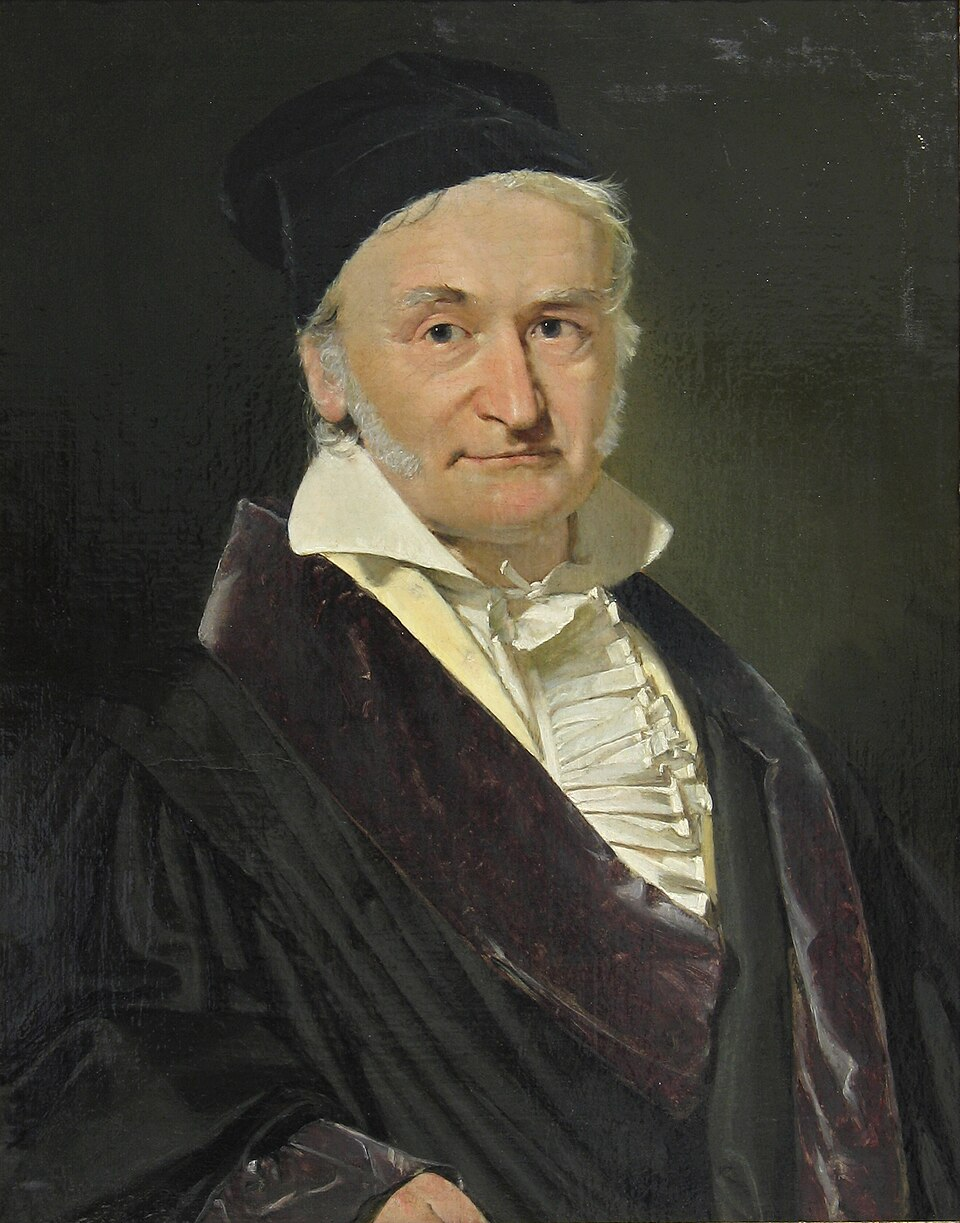
\includegraphics[height=0.56\textheight]{ch2_gauss_1840.jpg}\\[1mm]
\imgcap{Carl Friedrich Gauss (1777--1855)}
\imgcredit{https://commons.wikimedia.org/wiki/File:Carl_Friedrich_Gauss_1840_by_Jensen.jpg}{Portrait: Christian Albrecht Jensen (1840); public domain; Wikimedia Commons}
\end{column}
\end{columns}
\end{frame}

\begin{frame}{The Normal Distribution: Definition}
\itemsize{\small}
\begin{itemize}
    \item $X \sim N(\mu, \sigma^2)$ has the \textbf{PDF} (probability density function)
    \begin{itemize}
        \item $f(x) = \dfrac{1}{\sigma\sqrt{2\pi}} \exp\Big(-\dfrac{(x - \mu)^2}{2\sigma^2}\Big)$, \quad $x \in \mathbb{R}$
        \item two parameters: the mean $\mu$ (location) and the variance $\sigma^2$ (spread)
    \end{itemize}
    \item \textbf{Standard Normal distribution}: $Z = (X - \mu)/\sigma \sim N(0, 1)$
    \begin{itemize}
        \item its \textbf{CDF} (cumulative distribution function) is $\Phi(z) = P(Z \le z)$, with no closed form; tables or software
    \end{itemize}
    \item Probabilities of $X$ come from $Z$: $P(X \le x) = \Phi\big((x - \mu)/\sigma\big)$
    \item Quantile of order $\alpha$: $x_\alpha = \mu + \sigma z_\alpha$, the value with $P(X \le x_\alpha) = \alpha$
    \begin{itemize}
        \item $z_\alpha = \Phi^{-1}(\alpha)$: the quantile of $N(0, 1)$; $z_{0.01} = -2.33$, $z_{0.05} = -1.64$
    \end{itemize}
\end{itemize}
\end{frame}

\begin{frame}{Properties Used in Finance}
\itemsize{\small}
\begin{itemize}
    \item Symmetric around $\mu$: mean = median = mode
    \item Skewness $0$ and kurtosis $3$ (defined in Section 5)
    \item \textbf{Closed under addition}: if $X \sim N(\mu_1, \sigma_1^2)$ and $Y \sim N(\mu_2, \sigma_2^2)$ are independent, then $X + Y \sim N(\mu_1 + \mu_2, \sigma_1^2 + \sigma_2^2)$
    \begin{itemize}
        \item $h$-day log return under the benchmark: $r_t(h) \sim N(h\mu, h\sigma^2)$
        \item volatility grows with $\sqrt{h}$: the square-root-of-time rule used in \sfmchlink{https://danpele.github.io/SFM/EN/Courses/chapter1_data_returns_indicators.pdf}{Chapter 1}
    \end{itemize}
    \item Linear combinations of jointly Normal returns are Normal, so portfolio returns stay Normal
    \item Fully described by two numbers: once $\mu$ and $\sigma$ are known, every probability is known
\end{itemize}
\end{frame}

\begin{frame}{The 68--95--99.7 Rule}
\itemsize{\footnotesize}
\begin{center}
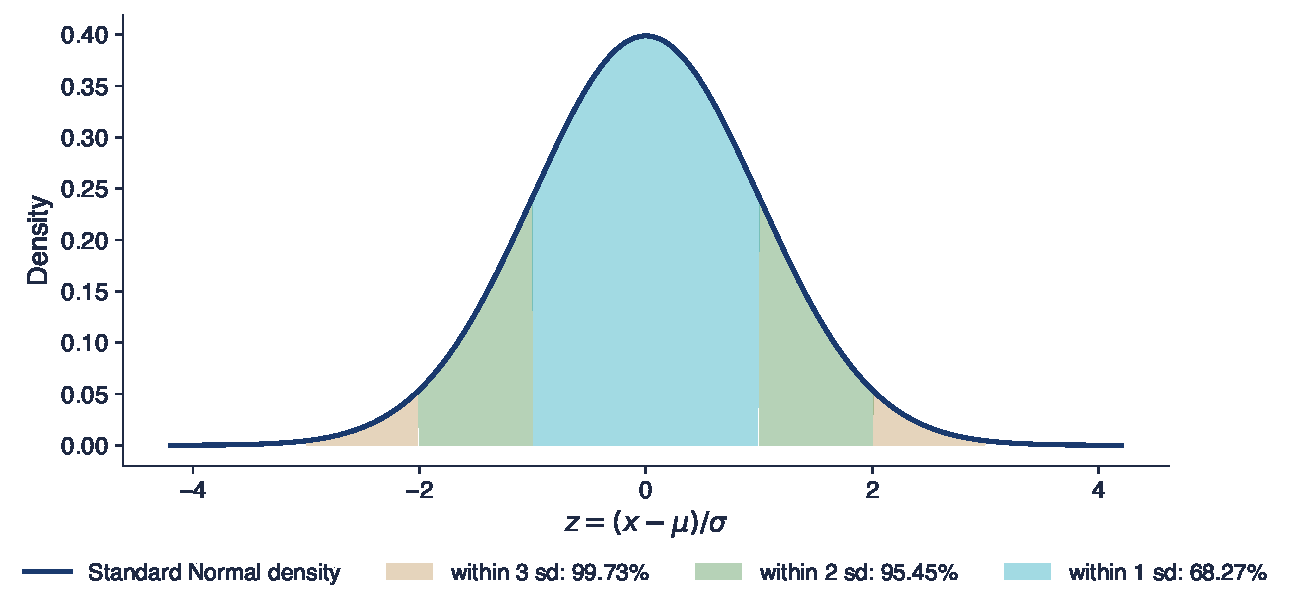
\includegraphics[width=0.97\textwidth,height=0.62\textheight,keepaspectratio]{sfm_ch2_normal_pdf.pdf}
\end{center}
\vspace{-0.25cm}
\begin{itemize}
    \item Within 1, 2 and 3 standard deviations: 68.27\%, 95.45\% and 99.73\% of the probability
    \item Outside 3 standard deviations: one day in 370; the tails of the Normal distribution fall off like $e^{-z^2/2}$, very fast
\end{itemize}
\sfmquantlet{Ch_02}{SFM_ch2_normal_lognormal}
\end{frame}

\begin{frame}{How Rare Are Large Moves under the Normal Distribution?}
\itemsize{\small}
\begin{center}
\footnotesize
\begin{tabular}{crrr}
\toprule
$k$ & $P(|Z| > k)$ & once every \dots\ trading days & once every \dots\ years \\
\midrule
1 & ${0.3173}$ & 3 & 0.013 \\
2 & ${0.0455}$ & 22 & 0.087 \\
3 & ${2.7 \times 10^{-3}}$ & 370 & 1.5 \\
4 & ${6.3 \times 10^{-5}}$ & 15\,787 & 63 \\
5 & ${5.7 \times 10^{-7}}$ & 1\,744\,278 & 6\,922 \\
6 & ${2.0 \times 10^{-9}}$ & 506\,797\,346 & 2\,011\,101 \\
\bottomrule
\end{tabular}
\end{center}
\begin{itemize}
    \item $P(|Z| > k)$: the probability that a standard Normal variable lies more than $k$ standard deviations from 0
    \item Years computed with 252 trading days a year
    \item Each extra standard deviation makes a move 7 to 291 times rarer
    \item A 6-sigma day should not happen in the whole history of stock markets
\end{itemize}\sfmquantlet{Ch_02}{SFM_ch2_normal_lognormal}
\end{frame}

\begin{frame}{Worked Example: Large Losses of the S\&P 500}
\itemsize{\footnotesize}
\begin{itemize}
    \item S\&P 500, 2010--2026: $n = 4\,201$ daily log returns, mean $0.045\%$, standard deviation $1.08\%$
    \item A loss larger than 3\%: $z = (-3 - 0.045)/1.08 = -2.81$
    \begin{itemize}
        \item Normal distribution: $\Phi(-2.81) = 0.25\%$, so $10.5$ days expected
        \item observed: 49 days
    \end{itemize}
    \item A loss larger than 5\%: $z = -4.65$
    \begin{itemize}
        \item Normal distribution: $6.9 \times 10^{-3}$ days expected; observed: 8 days
    \end{itemize}
    \item BET: 13 days below $-5\%$ against $5.1 \times 10^{-3}$ expected
    \item The Normal distribution underestimates the frequency of large losses by orders of magnitude
\end{itemize}
\end{frame}

\begin{frame}{Recap: The Normal Distribution}
\itemsize{\small}
\begin{itemize}
    \item Two parameters, symmetric, closed under addition, volatility scales with $\sqrt{h}$
    \item Its tails are thin: a 4-sigma day once every 63 years
    \item Real returns have many more large moves than it allows
\end{itemize}
\end{frame}


%=============================================================================
\section{The Lognormal Distribution}
%=============================================================================

\begin{frame}{From Normal Log Returns to Lognormal Prices}
\itemsize{\small}
\begin{itemize}
    \item A positive variable $Y$ is \textbf{lognormal}, $Y \sim LN(m, s^2)$, if $\ln Y \sim N(m, s^2)$
    \begin{itemize}
        \item $m$, $s^2$: the mean and the variance of $\ln Y$, not of $Y$
    \end{itemize}
    \item Density: $f(y) = \dfrac{1}{y s\sqrt{2\pi}} \exp\Big(-\dfrac{(\ln y - m)^2}{2s^2}\Big)$, \quad $y > 0$
    \item Under the benchmark, $\ln(P_T/P_0) = r_1 + \dots + r_T \sim N(T\mu, T\sigma^2)$
    \begin{itemize}
        \item $T$: the horizon in days; so $P_T/P_0 \sim LN(T\mu, T\sigma^2)$ \refOsborne
    \end{itemize}
    \item Why lognormal and not Normal prices?
    \begin{itemize}
        \item prices cannot be negative; a Normal price could be
        \item the simple return $R = e^r - 1 > -1$: you cannot lose more than you invested
    \end{itemize}
    \item The Black--Scholes model is built on it
\end{itemize}
\end{frame}

\begin{frame}{Mean, Median and Mode}
\itemsize{\small}
\begin{itemize}
    \item If $Y \sim LN(m, s^2)$:
    \item median $e^{m}$; mode $e^{m - s^2}$; mean $E[Y] = e^{m + s^2/2}$
    \begin{itemize}
        \item mode: the most likely value; median: the value exceeded with probability 1/2
        \item always mode $<$ median $<$ mean: a long right tail (positive skewness)
    \end{itemize}
    \item Variance: $\text{Var}(Y) = (e^{s^2} - 1)\,e^{2m + s^2}$
    \item The mean comes from $E[e^X] = e^{m + s^2/2}$ for $X \sim N(m, s^2)$ (Seminar 2 derives it)
    \begin{itemize}
        \item the extra $s^2/2$ is the volatility drag of \sfmchlink{https://danpele.github.io/SFM/EN/Courses/chapter1_data_returns_indicators.pdf}{Chapter 1}, seen from the other side
    \end{itemize}
    \item Which one matters? The median is the outcome of a typical investor; the mean is pulled up by a few very good paths
\end{itemize}
\end{frame}

\begin{frame}{Lognormal Densities (SFElognormal)}
\itemsize{\footnotesize}
\begin{center}
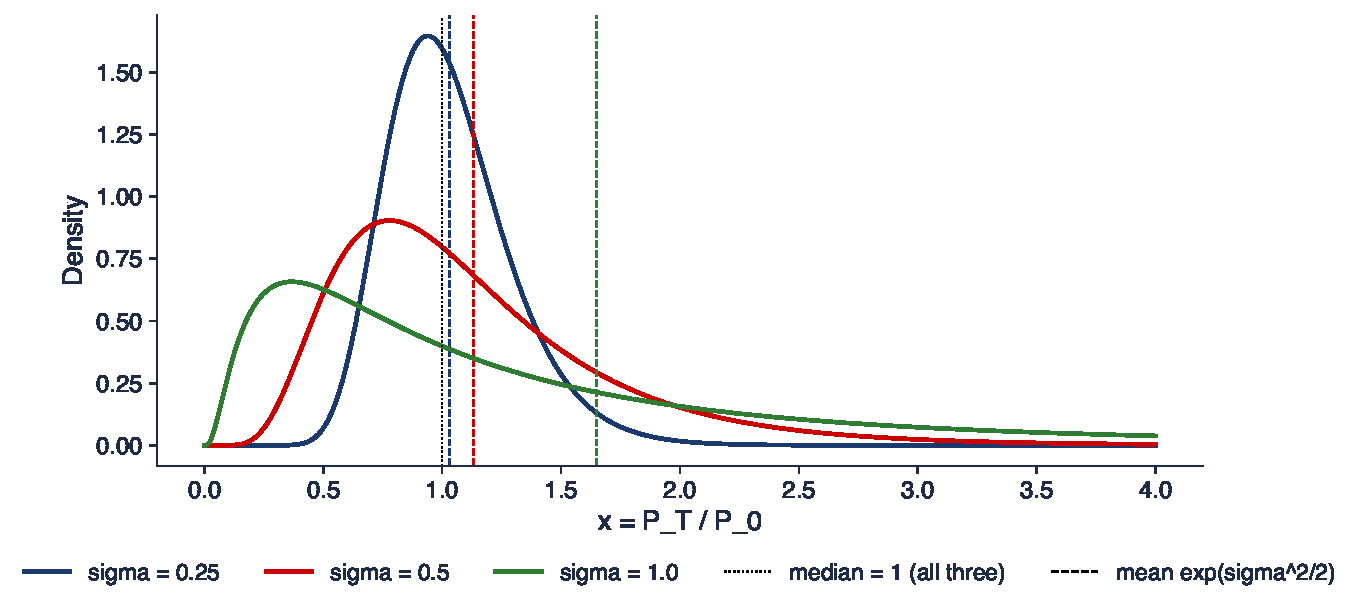
\includegraphics[width=0.97\textwidth,height=0.62\textheight,keepaspectratio]{sfm_ch2_lognormal.pdf}
\end{center}
\vspace{-0.25cm}
\begin{itemize}
    \item $m = 0$: the median is 1 for all three curves; the dashed lines mark the means
    \item $s = 0.25$: mean $1.03$, mode $0.94$, almost symmetric; $s = 1$: mean $1.65$, mode $0.37$, skewness $6.18$
    \item Long horizons or high volatility: the gap between mean and median widens
\end{itemize}
\sfmquantlet{Ch_02}{SFM_ch2_normal_lognormal}
\end{frame}

\begin{frame}{Worked Example: 100 Lei in the BET}
\itemsize{\footnotesize}
\begin{itemize}
    \item BET, 2010--2026: annual mean log return $\mu = 11.6\%$ and volatility $\sigma = 16.9\%$ (daily moments $\times$ 251 and $\sqrt{251}$)
    \item After 1 year, $P_1/P_0 \sim LN(\mu, \sigma^2)$
    \begin{itemize}
        \item median $100e^{\mu} = 112.3$; mean $100e^{\mu + \sigma^2/2} = 113.9$
        \item probability of a loss $\Phi(-\mu/\sigma) = 24.8\%$; 5\% quantile $100e^{\mu - 1.645\sigma} = 84.9$
        \item $\Phi(-\mu/\sigma) = P(r < 0)$: the probability of a negative log return; $-1.645 = z_{0.05}$
    \end{itemize}
    \item After 10 years, $P_{10}/P_0 \sim LN(10\mu, 10\sigma^2)$
    \begin{itemize}
        \item median 317.7; mean 366.8; probability of a loss 1.5\%; 5\% quantile 131.6
    \end{itemize}
    \item The probability of a loss falls with the horizon; after 10 years even the 5\% quantile is above 100, but only if the historical mean persists
    \item Caveat: these numbers inherit every weakness of the Normal model of log returns
\end{itemize}
\end{frame}

\begin{frame}{Recap: The Lognormal Distribution}
\itemsize{\small}
\begin{itemize}
    \item Normal log returns $\Rightarrow$ lognormal prices: positive, right-skewed
    \item Median $e^m$ below mean $e^{m + s^2/2}$: the gap is the volatility drag
    \item Report the median and a low quantile, not only the mean
\end{itemize}
\end{frame}


%=============================================================================
\section{The Central Limit Theorem}
%=============================================================================

\begin{frame}{The Galton Board}
\itemsize{\small}
\begin{columns}[T]
\begin{column}{0.52\textwidth}
\begin{itemize}
    \item Francis Galton (1889): balls fall through rows of pins and bounce left or right with probability $1/2$
    \item The final position of a ball is a \textbf{sum} of many small independent shocks
    \item The heaps form a bell curve: binomial probabilities close to the Normal density
    \item The same argument was used for returns: a daily return is the sum of many small price changes during the day
\end{itemize}
\end{column}
\begin{column}{0.44\textwidth}
\centering
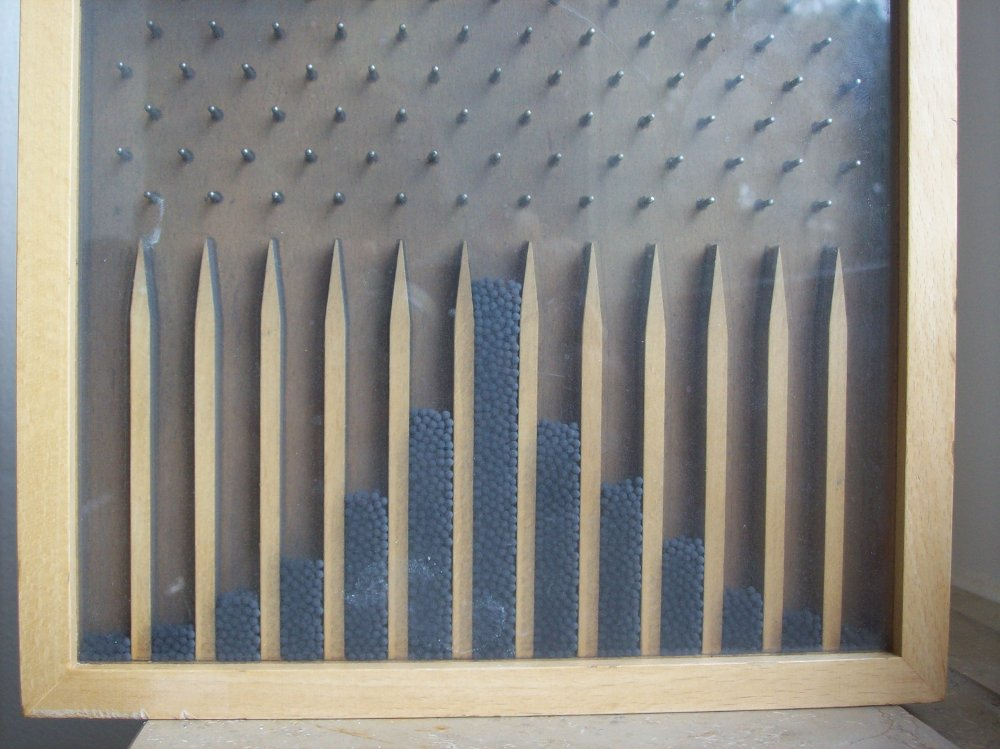
\includegraphics[height=0.45\textheight]{ch2_galton_board.jpg}\\[1mm]
\imgcap{A Galton board after the balls have fallen}
\imgcredit{https://commons.wikimedia.org/wiki/File:Galton_box_2.jpg}{Photo: Klaus-Dieter Keller (2010); public domain; Wikimedia Commons}
\end{column}
\end{columns}
\end{frame}

\begin{frame}{The Central Limit Theorem}
\itemsize{\small}
\begin{itemize}
    \item \textbf{CLT} (Lindeberg--Lévy): $X_1, \dots, X_n$ i.i.d. with mean $\mu$ and finite variance $\sigma^2$
    \begin{itemize}
        \item $\dfrac{\sqrt{n}\,(\bar X_n - \mu)}{\sigma} \xrightarrow{d} N(0, 1)$ as $n \to \infty$
        \item $\bar X_n$: the mean of the $n$ variables; $\xrightarrow{d}$: convergence in distribution, the CDF of the left side approaches $\Phi$
        \item equivalently, the sum $X_1 + \dots + X_n$ is approximately $N(n\mu, n\sigma^2)$
    \end{itemize}
    \item Three conditions
    \begin{itemize}
        \item independence; identical distribution; finite variance
    \end{itemize}
    \item How fast? The error falls like $1/\sqrt{n}$ and grows with the skewness of $X$ (Berry--Esseen bound)
    \item It explains why the Normal distribution is everywhere, and why sample means have Normal confidence intervals
\end{itemize}
\end{frame}

\begin{frame}{The CLT at Work (SFEclt)}
\itemsize{\footnotesize}
\begin{center}
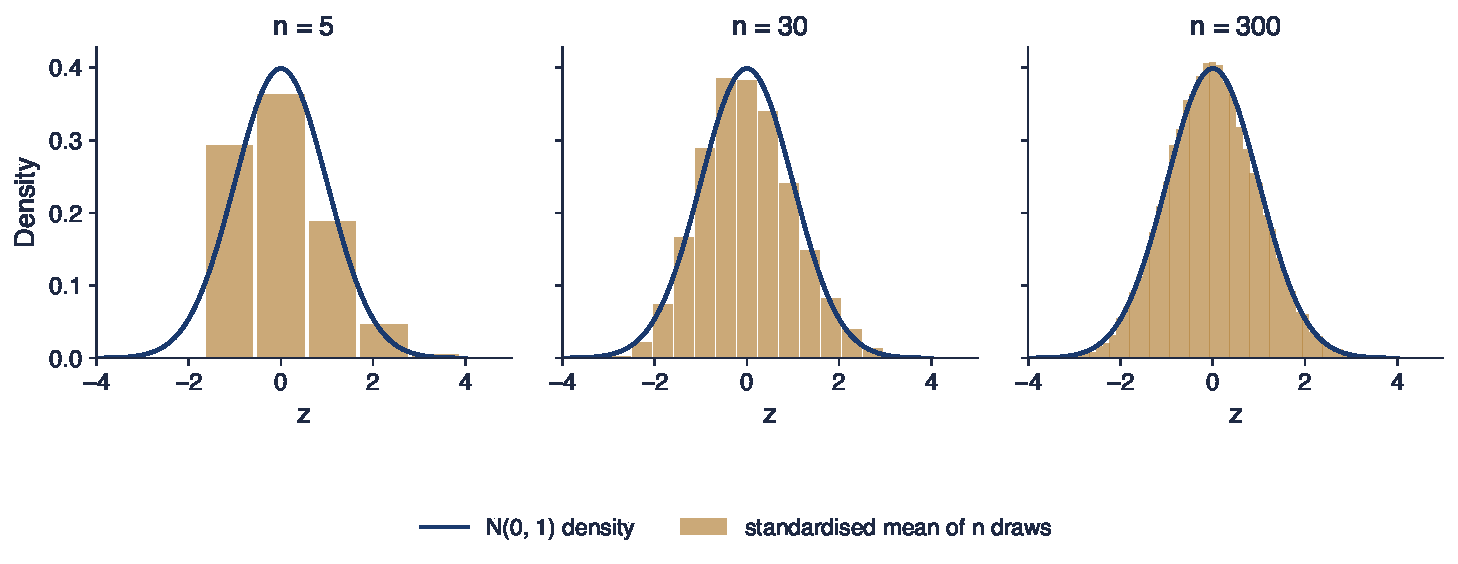
\includegraphics[width=0.97\textwidth,height=0.60\textheight,keepaspectratio]{sfm_ch2_clt.pdf}
\end{center}
\vspace{-0.25cm}
\begin{itemize}
    \item Standardised mean of $n$ Bernoulli($0.2$) draws (a skewed variable), 20\,000 simulations
    \item Share above $1.96$: 5.8\% for $n = 5$, 2.7\% for $n = 30$, 2.8\% for $n = 300$; Normal distribution: 2.5\%
    \item Skewness of the mean, $(1 - 2p)/\sqrt{np(1-p)}$ with $p = 0.2$: $0.67$, $0.27$, $0.09$; it falls like $1/\sqrt{n}$
\end{itemize}
\sfmquantlet{Ch_02}{SFM_ch2_clt_normal_approx}
\end{frame}

\begin{frame}{The Normal Approximation of the Binomial (SFENormalApprox)}
\itemsize{\footnotesize}
\begin{center}
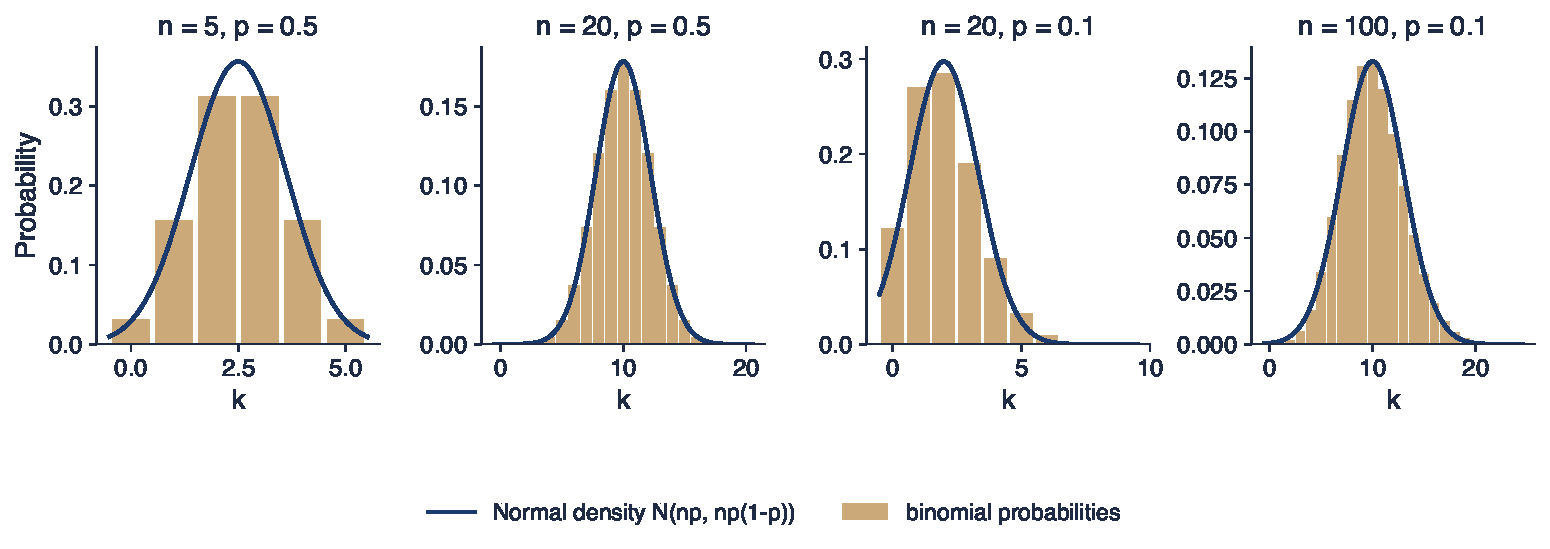
\includegraphics[width=0.97\textwidth,height=0.54\textheight,keepaspectratio]{sfm_ch2_normal_approx.pdf}
\end{center}
\vspace{-0.25cm}
\begin{itemize}
    \item $B(n, p)$: the number of successes in $n$ independent trials with success probability $p$; $B(n, p) \approx N\big(np, np(1-p)\big)$
    \item Continuity correction: $P(X \le k) \approx \Phi\big((k + 0.5 - np)/\sqrt{np(1-p)}\big)$; the $+0.5$ spreads each integer $k$ over $[k - 0.5, k + 0.5]$
    \item Largest error of the CDF: $0.001$ for $n = 20, p = 0.5$; $0.037$ for $n = 20, p = 0.1$; $0.017$ for $n = 100, p = 0.1$
    \item Rule of thumb: the approximation is good when $np(1-p)$ is large (at least about 9)
\end{itemize}
\sfmquantlet{Ch_02}{SFM_ch2_clt_normal_approx}
\end{frame}

\begin{frame}{Question for the Room: Does the CLT Make Daily Returns Normal?}
\itemsize{\small}
\begin{itemize}
    \item A daily log return is the sum of thousands of intraday log returns
    \item \textbf{What do you think?} Should daily returns then be close to the Normal distribution?
    \item \textbf{Answer}: not necessarily; each condition of the CLT can fail
    \begin{itemize}
        \item dependence: calm and turbulent days come in clusters (Section 8)
        \item changing distribution: volatility differs from day to day
        \item infinite variance: \refMandelbrot{} proposed it for cotton prices (\sfmchlink{https://danpele.github.io/SFM/EN/Courses/chapter3_alpha_stable_distributions.pdf}{Chapter 3}, $\alpha$-stable distributions)
    \end{itemize}
    \item The data decide: the next sections measure how far returns are from the Normal distribution
\end{itemize}
\end{frame}

\begin{frame}{Recap: The Central Limit Theorem}
\itemsize{\small}
\begin{itemize}
    \item Sums of many i.i.d. terms with finite variance are approximately Normal
    \item Convergence is slower for skewed variables; $np(1-p) \ge 9$ for the binomial
    \item Returns may violate independence, identical distribution or finite variance
\end{itemize}
\end{frame}


%=============================================================================
\section{Moments and the Shape of a Distribution}
%=============================================================================

\begin{frame}{Four Moments}
\itemsize{\small}
\begin{itemize}
    \item Mean $\mu = E[X]$; variance $\sigma^2 = E[(X - \mu)^2]$; $E[\cdot]$ is the expected value
    \item \textbf{Skewness}: $\gamma_1 = E[(X - \mu)^3]/\sigma^3$
    \begin{itemize}
        \item the third power keeps the sign of each deviation; $\gamma_1 < 0$: a longer left tail, large losses more frequent than large gains
    \end{itemize}
    \item \textbf{Kurtosis}: $\gamma_2 = E[(X - \mu)^4]/\sigma^4$; Normal distribution: $\gamma_2 = 3$
    \begin{itemize}
        \item \textbf{excess kurtosis} $\gamma_2 - 3$: positive means heavy tails and a tall, narrow centre (\textbf{leptokurtic})
    \end{itemize}
    \item Both are free of units: they describe the shape, not the location or the scale
    \item Fourth powers make the kurtosis very sensitive to a few extreme days
\end{itemize}
\end{frame}

\begin{frame}{What Skewness and Kurtosis Look Like}
\itemsize{\footnotesize}
\begin{center}
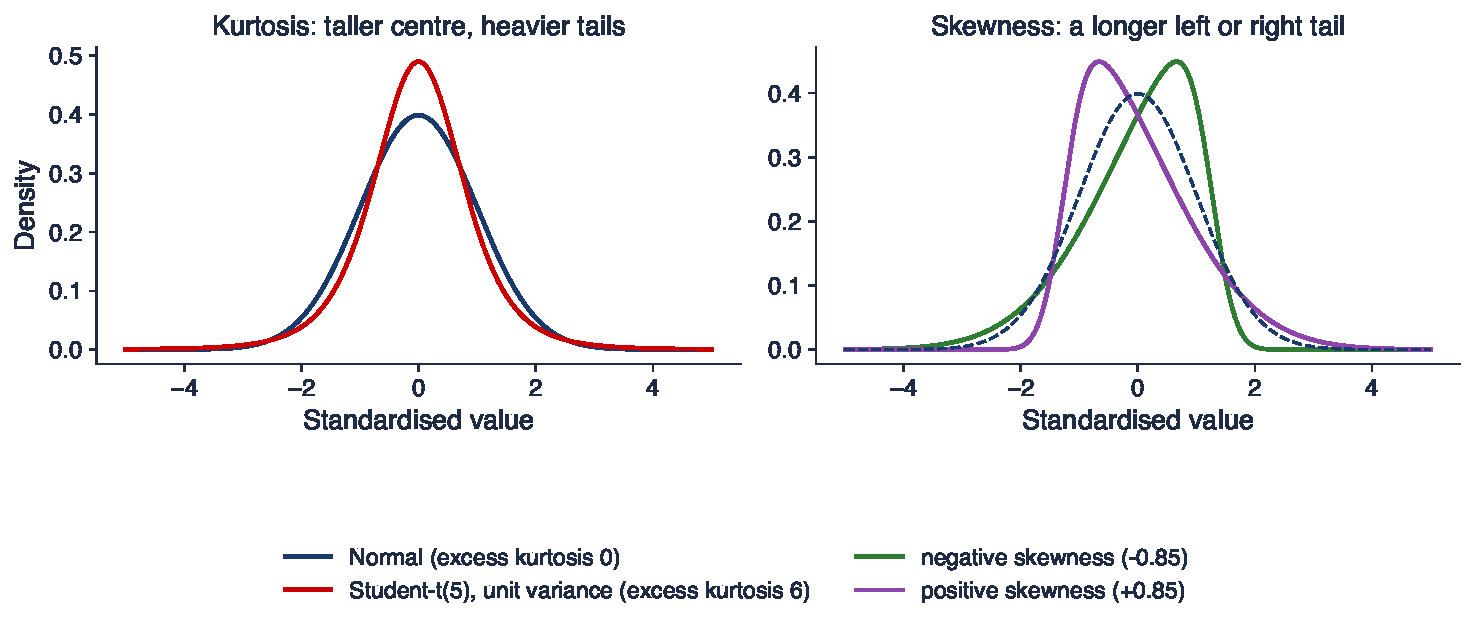
\includegraphics[width=0.97\textwidth,height=0.62\textheight,keepaspectratio]{sfm_ch2_shapes.pdf}
\end{center}
\vspace{-0.25cm}
\begin{itemize}
    \item Left: same mean and variance; the Student-$t(5)$ curve (Section 7) has excess kurtosis 6: more mass in the centre and in the tails, less in the shoulders
    \item Right: skew-Normal densities with skewness $\pm 0.85$; the dashed curve is the Normal distribution
\end{itemize}
\sfmquantlet{Ch_02}{SFM_ch2_moments_jarque_bera}
\end{frame}

\begin{frame}{Sample Moments}
\itemsize{\small}
\begin{itemize}
    \item Central sample moments: $m_k = \frac1n \sum_{t=1}^n (r_t - \bar r)^k$, the average $k$-th power of the deviations from the mean ($m_2$: variance)
    \item Sample skewness $S = m_3/m_2^{3/2}$; sample excess kurtosis $K = m_4/m_2^2 - 3$
    \item If the data are i.i.d. Normal: $S \approx N(0, 6/n)$ and $K \approx N(0, 24/n)$
    \begin{itemize}
        \item with $n = 4\,201$: standard errors $\sqrt{6/n} = 0.038$ and $\sqrt{24/n} = 0.076$
    \end{itemize}
    \item These standard errors hold only under normality; for heavy-tailed data they are far too small (Seminar 2, B1)
\end{itemize}
\end{frame}

\begin{frame}{Daily Log Returns: Moments, 2010--2026}
\itemsize{\footnotesize}
\begin{center}
\footnotesize
\begin{tabular}{lrrrrrrr}
\toprule
Series & from & $n$ & Mean \% & S.d. \% & Skew. & Exc. kurt. & Min \% \\
\midrule
S\&P 500 & 2010 & 4\,201 & $0.045$ & $1.08$ & $-0.61$ & $13.5$ & $-12.8$ \\
DAX & 2010 & 4\,244 & $0.034$ & $1.22$ & $-0.45$ & $7.4$ & $-13.1$ \\
BET & 2010 & 4\,186 & $0.046$ & $1.07$ & $-0.98$ & $17.9$ & $-11.9$ \\
Bitcoin & 2014 & 4\,384 & $0.118$ & $3.49$ & $-0.70$ & $12.0$ & $-46.5$ \\
OMV Petrom (SNP) & 2010 & 3\,815 & $0.076$ & $1.62$ & $-0.54$ & $8.9$ & $-15.8$ \\
BRD & 2010 & 3\,771 & $0.044$ & $1.66$ & $-0.38$ & $7.3$ & $-18.2$ \\
Nuclearelectrica (SNN) & 2013 & 2\,911 & $0.099$ & $1.52$ & $0.27$ & $5.1$ & $-9.4$ \\
Romgaz (SNG) & 2013 & 2\,909 & $0.090$ & $1.40$ & $-0.34$ & $5.3$ & $-11.0$ \\
\bottomrule
\end{tabular}
\end{center}
\begin{itemize}
    \item Every series has excess kurtosis between 5.1 (SNN) and 17.9 (BET): far from 0
    \item Every series except SNN has negative skewness
    \item Worst days: S\&P 500 on 16 March 2020, BET on 19 December 2018 (OUG 114, a tax on bank assets), Bitcoin on 12 March 2020
\end{itemize}\sfmquantlet{Ch_02}{SFM_ch2_moments_jarque_bera}
\end{frame}

\begin{frame}{DAX Returns vs the Normal Density (SFEDaxReturnDistribution)}
\itemsize{\footnotesize}
\begin{center}
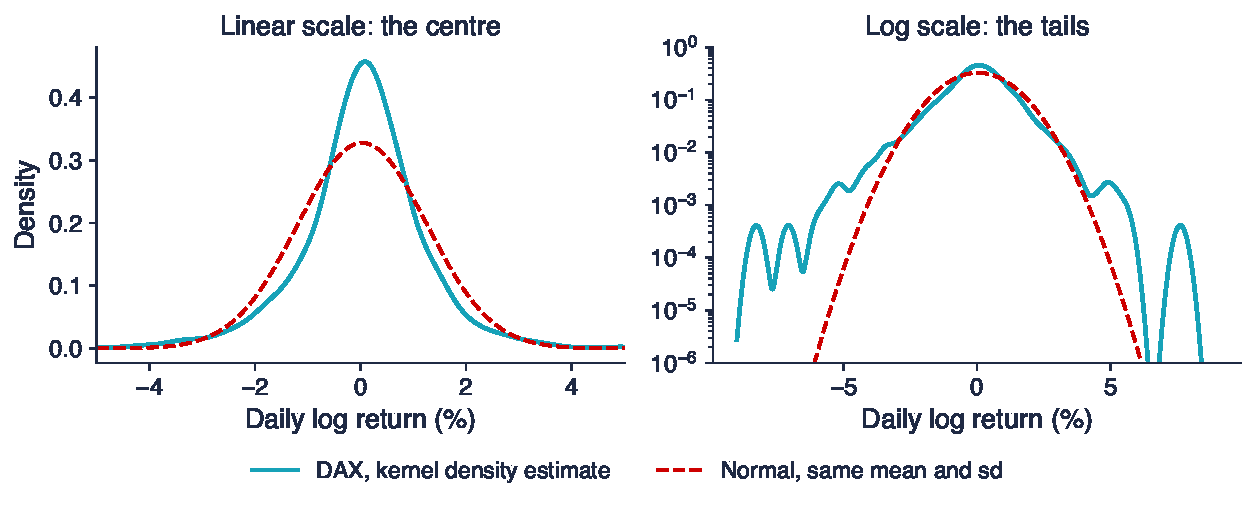
\includegraphics[width=0.97\textwidth,height=0.60\textheight,keepaspectratio]{sfm_ch2_dax_density.pdf}
\end{center}
\vspace{-0.25cm}
\begin{itemize}
    \item Kernel density estimate (a smoothed histogram) against the Normal density with the same mean and standard deviation
    \item Centre: peak 0.46 vs 0.33; 76.8\% of days within one standard deviation, vs 68.3\% for the Normal distribution
    \item Tails (log scale): at $-6\%$ the estimated density is 439 times the Normal one
\end{itemize}
\sfmquantlet{Ch_02}{SFM_ch2_moments_jarque_bera}
\end{frame}

\begin{frame}{Check the Data Before Measuring Tails}
\itemsize{\footnotesize}
\begin{itemize}
    \item Banca Transilvania (TLV), 27--31 May 2016: the close falls from 2.83 to 2.09 lei, the ex-date of a bonus share issue
    \item The adjusted close in our data: 3.60, then 3.10, then 3.81
    \begin{itemize}
        \item log returns $-15.0\%$ and $+20.5\%$ on two consecutive days: the adjustment was applied one day late
    \end{itemize}
    \item Excess kurtosis of TLV, 2010--2026: 17.5 with these two days, 13.5 without them
    \item Two wrong days out of thousands change the kurtosis by a third: this is why TLV is not in the tables of this chapter
    \item Rule from \sfmchlink{https://danpele.github.io/SFM/EN/Courses/chapter1_data_returns_indicators.pdf}{Chapter 1}: list the largest moves and check each one, especially pairs of opposite jumps
\end{itemize}
\end{frame}

\begin{frame}{Recap: Moments}
\itemsize{\small}
\begin{itemize}
    \item Skewness measures asymmetry, excess kurtosis measures tail weight relative to the Normal distribution
    \item Daily returns: mostly negative skewness and excess kurtosis between 5 and 18
    \item Kurtosis is driven by a few days: check them before trusting it
\end{itemize}
\end{frame}


%=============================================================================
\section{Testing Normality: Jarque--Bera and QQ Plots}
%=============================================================================

\begin{frame}{The Jarque--Bera Test}
\itemsize{\small}
\begin{itemize}
    \item $H_0$: the data are Normal, so skewness $= 0$ and excess kurtosis $= 0$
    \item \textbf{JB} statistic \refJBa, \refJBb: $\text{JB} = \dfrac{n}{6}\Big(S^2 + \dfrac{K^2}{4}\Big)$
    \begin{itemize}
        \item the sum of two squared standardised statistics: $(S/\sqrt{6/n})^2 + (K/\sqrt{24/n})^2$
    \end{itemize}
    \item Under $H_0$ and for large $n$: $\text{JB} \sim \chi^2(2)$; reject at 5\% if $\text{JB} > 5.99$
    \begin{itemize}
        \item $\chi^2(2)$: the chi-squared distribution with 2 degrees of freedom, the distribution of a sum of two squared independent $N(0,1)$ variables; 5.99 is its 95\% quantile
        \item JB $= 0$ for a perfect Normal shape; large values mean skewness or excess kurtosis far from 0
    \end{itemize}
    \item Simple, uses only two moments, and is the standard test reported in empirical finance
\end{itemize}
\end{frame}

\begin{frame}{Worked Example: Jarque--Bera for the S\&P 500}
\itemsize{\small}
\begin{itemize}
    \item $n = 4\,201$, $S = -0.61$, $K = 13.5$
    \item $\text{JB} = 700.2 \times (0.367 + 45.5) = 32\,113$
    \item Critical value 5.99: normality is rejected; the p-value is zero to any number of decimals
    \item The kurtosis term dominates: almost all of JB comes from $K^2/4$
    \item JB for the other series: all rejected at any usual level
    \begin{itemize}
        \item indices and Bitcoin: BET 56\,762, DAX 9\,909, Bitcoin 26\,482
        \item BVB stocks: SNP 12\,832, BRD 8\,370, SNN 3\,174, SNG 3\,415
    \end{itemize}
\end{itemize}
\end{frame}

\begin{frame}{What Jarque--Bera Does Not Tell You}
\itemsize{\small}
\begin{itemize}
    \item With thousands of observations it rejects even tiny departures
    \begin{itemize}
        \item report the size of $S$ and $K$, not only the p-value
    \end{itemize}
    \item It assumes i.i.d. data; with volatility clustering its standard errors are too small
    \begin{itemize}
        \item S\&P 500: Normal-theory 95\% interval for $K$: $[13.34, 13.64]$; bootstrap interval: $[6.7, 20.6]$ (Seminar 2, B1)
    \end{itemize}
    \item A rejection says the data are not Normal; it does not say which distribution they follow
    \item Other tests (Kolmogorov--Smirnov, Anderson--Darling) compare the whole CDF: \sfmchlink{https://danpele.github.io/SFM/EN/Courses/chapter6_model_selection_risk_management.pdf}{Chapter 6}
\end{itemize}
\end{frame}

\begin{frame}{QQ Plots}
\itemsize{\small}
\begin{itemize}
    \item A \textbf{QQ plot} (quantile--quantile plot) compares the empirical quantiles with those of a model \refWG
    \begin{itemize}
        \item sort the data: $r_{(1)} \le r_{(2)} \le \dots \le r_{(n)}$
        \item plot $r_{(i)}$ against the model quantile $F^{-1}\big((i - 0.5)/n\big)$
        \item $r_{(i)}$: the $i$-th smallest return; $F^{-1}$: the quantile function of the model; $(i - 0.5)/n$: the share of the data below $r_{(i)}$
    \end{itemize}
    \item Reading
    \begin{itemize}
        \item points on the 45-degree line: the model fits
        \item an S-shape, low end below and high end above the line: heavier tails than the model
        \item only one end bent away: skewness
    \end{itemize}
    \item Unlike JB, it shows \textbf{where} the model fails: centre, shoulders or tails
\end{itemize}
\end{frame}

\begin{frame}{QQ Plots against the Normal Distribution}
\itemsize{\footnotesize}
\begin{center}
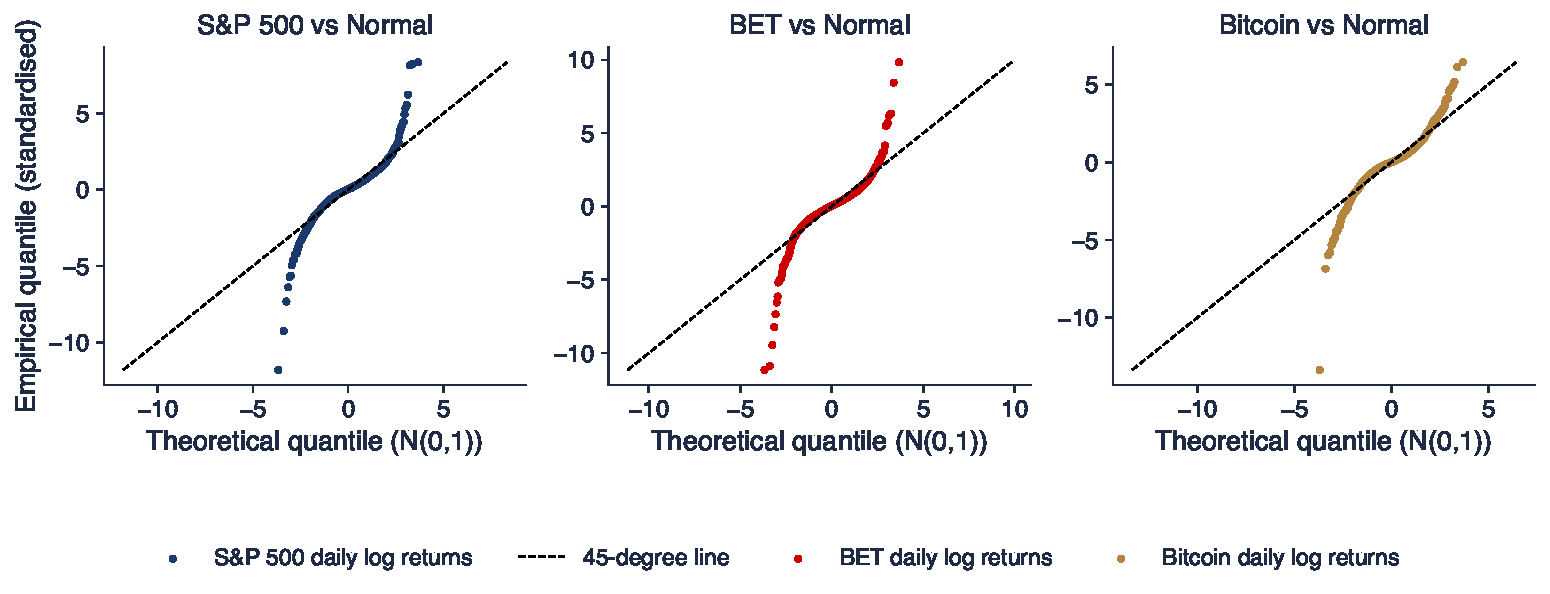
\includegraphics[width=0.97\textwidth,height=0.62\textheight,keepaspectratio]{sfm_ch2_qq_normal.pdf}
\end{center}
\vspace{-0.25cm}
\begin{itemize}
    \item Standardised returns against $N(0,1)$ quantiles: all three bend away from the line at both ends
    \item S\&P 500: lowest standardised return $-11.8$ where the Normal quantile is $-3.7$; BET: $-11.2$ vs $-3.7$
    \item The lower tail bends more than the upper one: negative skewness
\end{itemize}
\sfmquantlet{Ch_02}{SFM_ch2_qq_plots}
\end{frame}

\begin{frame}{Recap: Testing Normality}
\itemsize{\small}
\begin{itemize}
    \item JB combines skewness and kurtosis; it rejects normality for every series
    \item Report the size of the departure; Normal-theory standard errors are too small
    \item QQ plots show where the model fails: here, in both tails
\end{itemize}
\end{frame}


%=============================================================================
\section{The Student-$t$ Distribution}
%=============================================================================

\begin{frame}{"Student": William Sealy Gosset}
\itemsize{\small}
\begin{columns}[T]
\begin{column}{0.58\textwidth}
\begin{itemize}
    \item Chemist and brewer at Guinness, Dublin, working with small samples of barley and hops
    \item The brewery did not allow its staff to publish under their own names: he signed ``Student'' \refStudent
    \item He derived the distribution of $(\bar X - \mu)/(s/\sqrt n)$ for Normal data: the $t$ distribution
    \item In finance it is used for a different reason: its tails are heavier than those of the Normal distribution \refPraetz, \refBG
\end{itemize}
\end{column}
\begin{column}{0.38\textwidth}
\centering
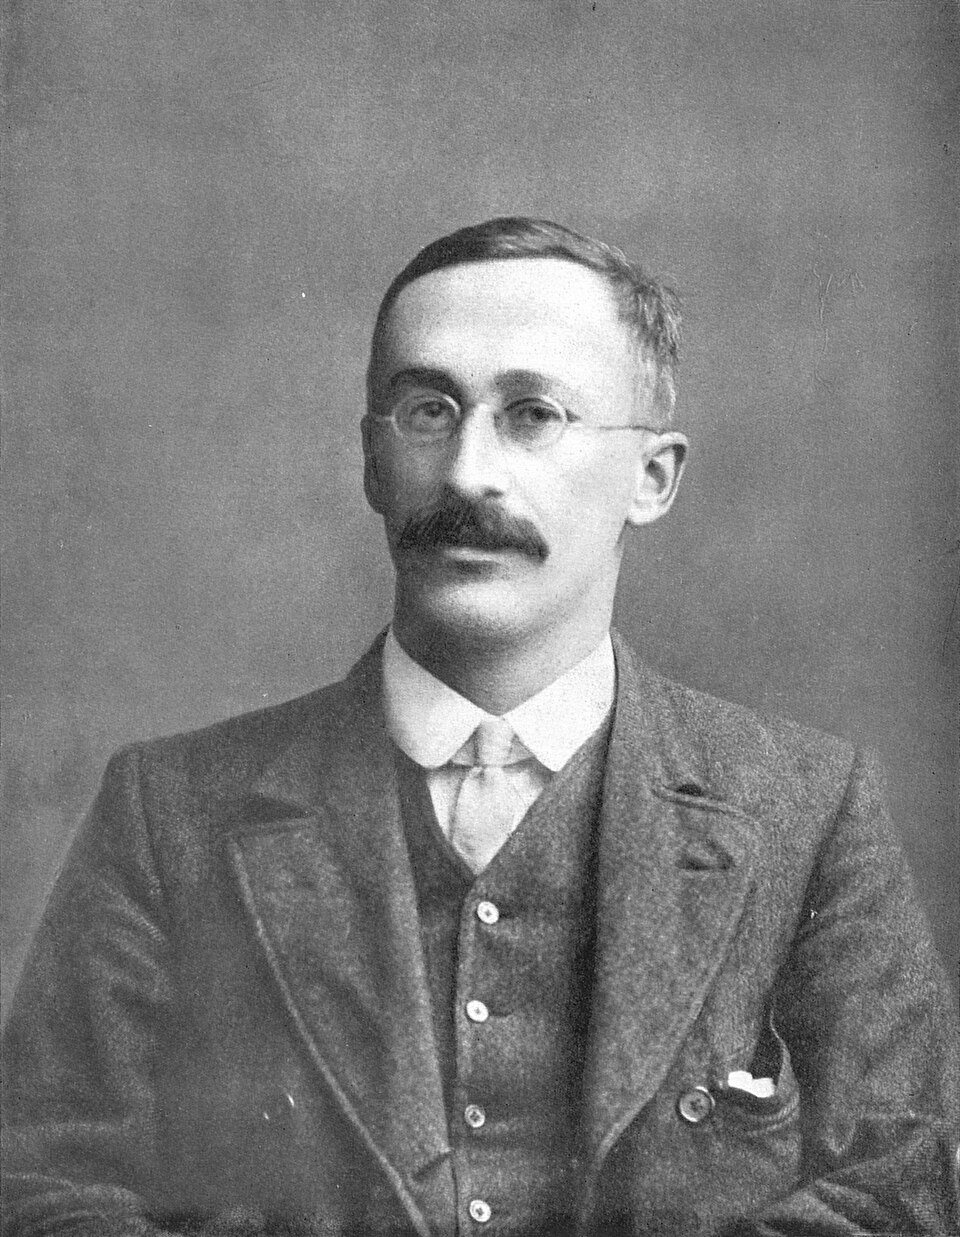
\includegraphics[height=0.56\textheight]{ch2_gosset_1908.jpg}\\[1mm]
\imgcap{William Sealy Gosset (1876--1937)}
\imgcredit{https://commons.wikimedia.org/wiki/File:William_Sealy_Gosset.jpg}{Photo: unknown author (1908); public domain; Wikimedia Commons}
\end{column}
\end{columns}
\end{frame}

\begin{frame}{The Student-$t$ Distribution: Definition}
\itemsize{\small}
\begin{itemize}
    \item $T = Z/\sqrt{V/\nu}$ with $Z \sim N(0,1)$ independent of $V \sim \chi^2(\nu)$: $T \sim t(\nu)$
    \begin{itemize}
        \item $\nu > 0$: the \textbf{degrees of freedom}, which control the tails
        \item $\chi^2(\nu)$: the distribution of a sum of $\nu$ squared independent $N(0,1)$ variables; $\Gamma$: the gamma function, $\Gamma(k) = (k-1)!$ for integer $k$
    \end{itemize}
    \item Density: $f(x) = \dfrac{\Gamma\big((\nu+1)/2\big)}{\sqrt{\nu\pi}\,\Gamma(\nu/2)} \Big(1 + \dfrac{x^2}{\nu}\Big)^{-(\nu+1)/2}$
    \item Location--scale version for returns: $r = m + s\,T$, with location $m$, scale $s$ and $\nu$
    \item As $\nu \to \infty$, $t(\nu) \to N(0,1)$: the Normal distribution is a limiting case
\end{itemize}
\end{frame}

\begin{frame}{Moments and Tails}
\itemsize{\small}
\begin{itemize}
    \item Mean $0$ if $\nu > 1$; variance $\nu/(\nu - 2)$ if $\nu > 2$; excess kurtosis $6/(\nu - 4)$ if $\nu > 4$
    \item Moments of order $\nu$ and higher are infinite
    \begin{itemize}
        \item $\nu \le 4$: infinite kurtosis; $\nu \le 2$: infinite variance
    \end{itemize}
    \item \textbf{Power-law tails}: $P(|T| > x) \approx c\,x^{-\nu}$ for large $x$
    \begin{itemize}
        \item $c > 0$: a constant; doubling $x$ divides the tail probability by about $2^{\nu}$
        \item the Normal tail falls like $e^{-x^2/2}$, much faster than any power
        \item $\nu$ is also the \textbf{tail index}, estimated directly in \sfmchlink{https://danpele.github.io/SFM/EN/Courses/chapter5_heavy_tails_evt.pdf}{Chapter 5}
    \end{itemize}
    \item To compare with the Normal distribution at the same variance, use $T\sqrt{(\nu - 2)/\nu}$, which has variance 1
\end{itemize}
\end{frame}

\begin{frame}{Student-$t$ Densities with Unit Variance}
\itemsize{\footnotesize}
\begin{center}
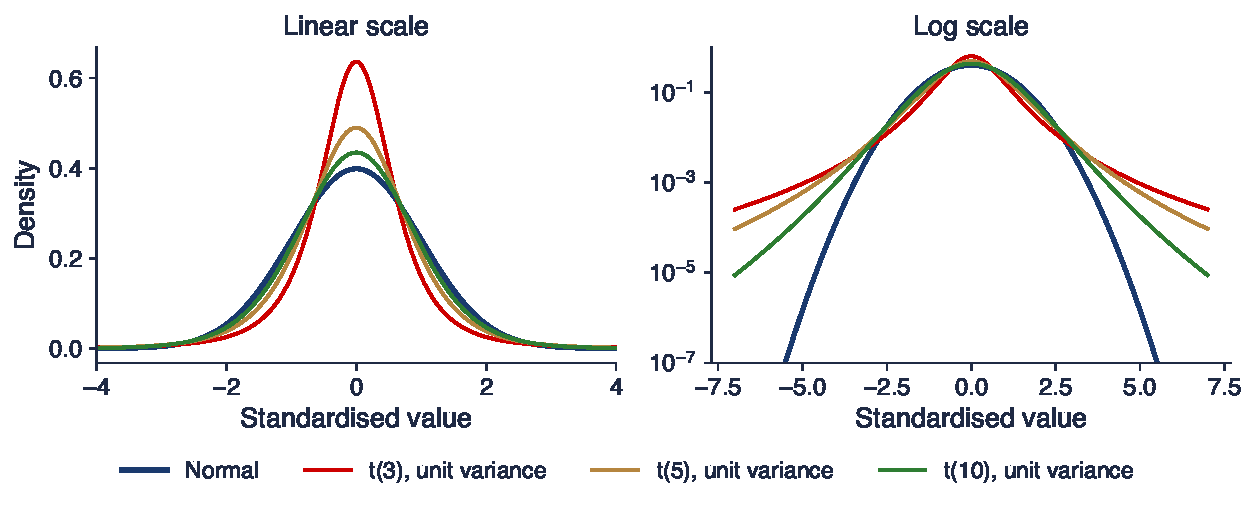
\includegraphics[width=0.97\textwidth,height=0.60\textheight,keepaspectratio]{sfm_ch2_t_densities.pdf}
\end{center}
\vspace{-0.25cm}
\begin{itemize}
    \item Smaller $\nu$: a taller centre and heavier tails; on the log scale the Normal tails drop like a parabola
    \item $P(|X| > 4)$ at unit variance: $t(3)$ 0.62\%, $t(5)$ 0.36\%, $t(10)$ 0.12\%, Normal distribution 0.0063\%
    \item With $\nu = 5$, a 4-sigma day is 56 times more likely than under the Normal distribution
\end{itemize}
\sfmquantlet{Ch_02}{SFM_ch2_student_t_fit}
\end{frame}

\begin{frame}{Fitting a Student-$t$ by Maximum Likelihood}
\itemsize{\small}
\begin{itemize}
    \item \textbf{MLE} (maximum likelihood estimation): choose $(\nu, m, s)$ that maximise the log-likelihood
    \begin{itemize}
        \item $\ell(\nu, m, s) = \sum_{t=1}^n \ln f\big((r_t - m)/s; \nu\big) - n \ln s$
        \item $f(\cdot; \nu)$: the $t(\nu)$ density; $-n \ln s$ corrects for rescaling the returns by $s$
        \item no closed form: a numerical optimiser (\texttt{scipy.stats.t.fit} in the notebook)
    \end{itemize}
    \item \textbf{AIC} (Akaike information criterion) \refAkaike: $\text{AIC} = 2k - 2\ell$
    \begin{itemize}
        \item $k$ = number of parameters (2 for the Normal distribution, 3 for the $t$); the lower AIC wins
        \item $\Delta\text{AIC} = \text{AIC}_{\text{Normal}} - \text{AIC}_{t} > 0$ favours the $t$
    \end{itemize}
    \item Early evidence for stock prices: \refPraetz, \refBG
\end{itemize}
\end{frame}

\begin{frame}{Fitted Student-$t$: Degrees of Freedom, 2010--2026}
\itemsize{\footnotesize}
\begin{columns}[T]
\begin{column}{0.55\textwidth}
\begin{center}
\footnotesize
\begin{tabular}{lrr}
\toprule
Series & $\hat\nu$ & $\Delta$AIC \\
\midrule
S\&P 500 & $2.78$ & $1213$ \\
DAX & $3.31$ & $739$ \\
BET & $2.96$ & $1454$ \\
Bitcoin & $2.23$ & $1335$ \\
OMV Petrom (SNP) & $3.79$ & $679$ \\
BRD & $4.67$ & $478$ \\
Nuclearelectrica (SNN) & $3.08$ & $541$ \\
Romgaz (SNG) & $3.40$ & $482$ \\
\bottomrule
\end{tabular}
\end{center}

\end{column}
\begin{column}{0.41\textwidth}
\begin{itemize}
    \item All $\hat\nu$ between 2.23 (Bitcoin) and 4.67 (BRD)
    \item $\hat\nu < 4$ for 7 of the 8 series: the fitted model has infinite kurtosis
    \item $\Delta$AIC is at least 478: the $t$ beats the Normal distribution everywhere
\end{itemize}
\end{column}
\end{columns}\sfmquantlet{Ch_02}{SFM_ch2_student_t_fit}
\end{frame}

\begin{frame}{S\&P 500: Normal vs Student-$t$ Fit}
\itemsize{\footnotesize}
\begin{center}
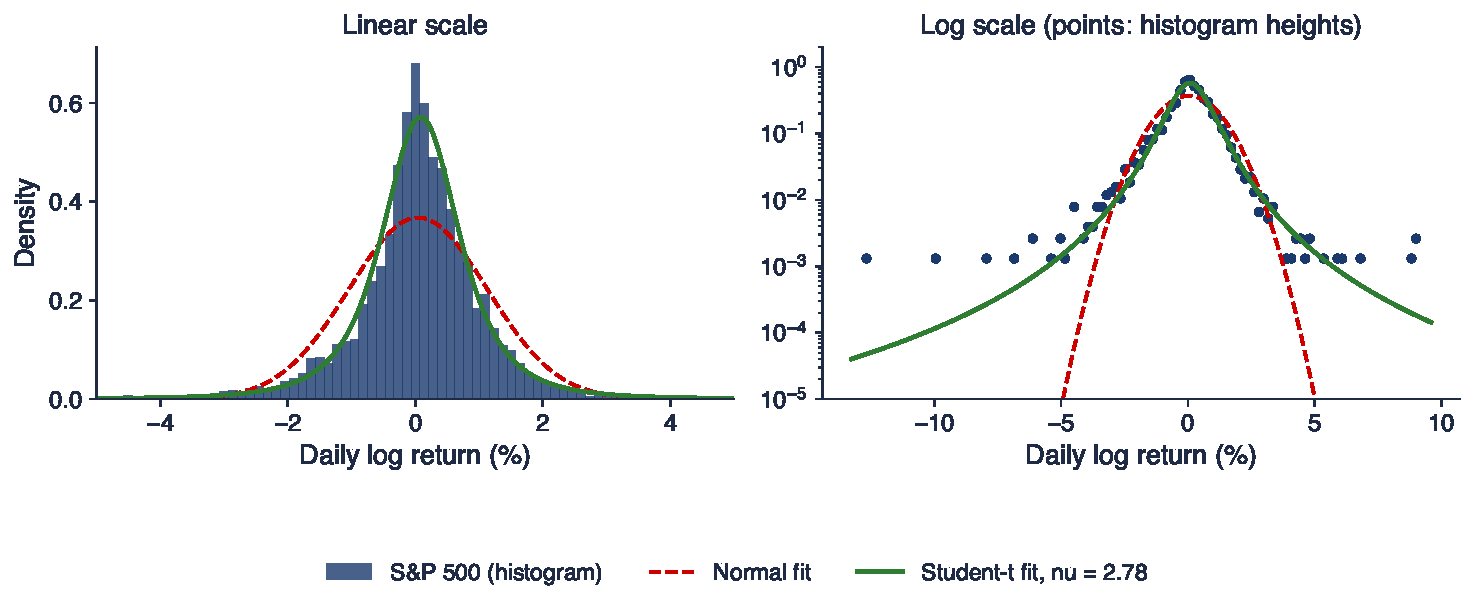
\includegraphics[width=0.97\textwidth,height=0.62\textheight,keepaspectratio]{sfm_ch2_t_fit_sp500.pdf}
\end{center}
\vspace{-0.25cm}
\begin{itemize}
    \item Linear scale: the $t$ ($\hat\nu = 2.78$) follows the tall centre that the Normal distribution misses
    \item Log scale: the Normal density collapses beyond $\pm 4\%$; the $t$ follows the observed tails
\end{itemize}
\sfmquantlet{Ch_02}{SFM_ch2_student_t_fit}
\end{frame}

\begin{frame}{QQ Plots against the Fitted Student-$t$}
\itemsize{\footnotesize}
\begin{center}
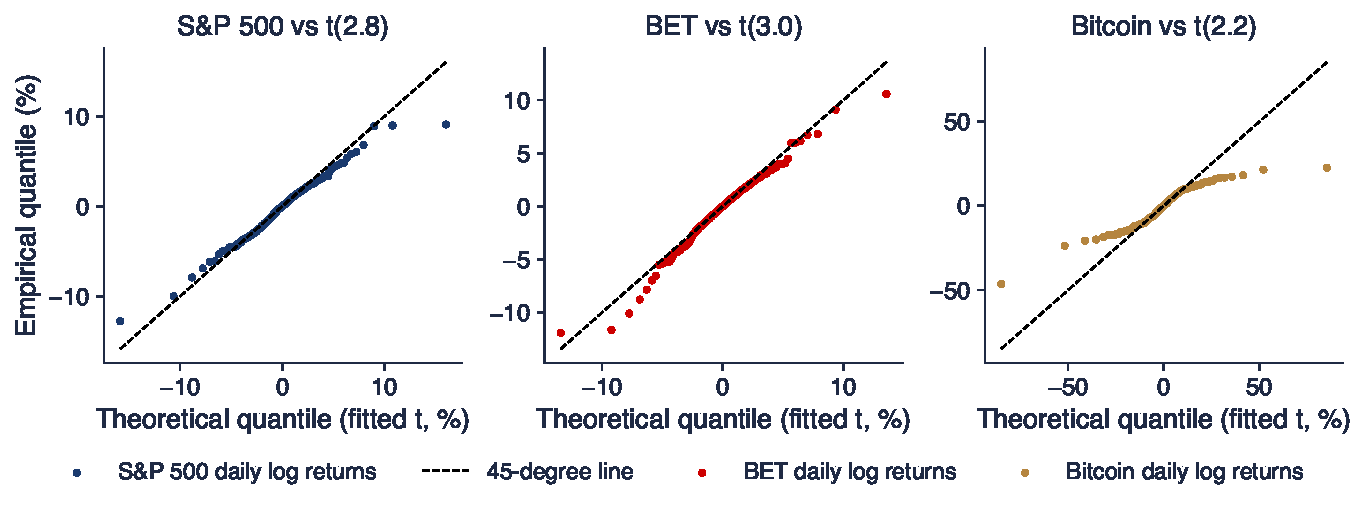
\includegraphics[width=0.97\textwidth,height=0.60\textheight,keepaspectratio]{sfm_ch2_qq_t.pdf}
\end{center}
\vspace{-0.25cm}
\begin{itemize}
    \item The centre and the moderate tails now lie on the line
    \item Extremes: the fitted $t$ expects lower minima than observed: S\&P 500 $-15.8\%$ vs $-12.8\%$; Bitcoin $-85.0\%$ vs $-46.5\%$
    \item With $\hat\nu$ close to 2 the model overshoots the most extreme quantiles
\end{itemize}
\sfmquantlet{Ch_02}{SFM_ch2_qq_plots}
\end{frame}

\begin{frame}{What the Student-$t$ Still Misses}
\itemsize{\small}
\begin{itemize}
    \item \textbf{Symmetry}: the $t$ cannot reproduce the negative skewness
    \begin{itemize}
        \item skewed $t$ distributions exist; they are beyond this chapter
    \end{itemize}
    \item \textbf{Independence}: an i.i.d. $t$ model has no volatility clustering
    \begin{itemize}
        \item GARCH models with $t$ errors combine both \refBollerslev{} (\sfmchlink{https://danpele.github.io/SFM/EN/Courses/chapter9_arch_garch_models.pdf}{Chapter 9})
    \end{itemize}
    \item \textbf{Single tail index}: one $\nu$ for both tails and for the centre
    \begin{itemize}
        \item extreme value theory models each tail separately (\sfmchlink{https://danpele.github.io/SFM/EN/Courses/chapter5_heavy_tails_evt.pdf}{Chapter 5})
    \end{itemize}
    \item Still the simplest heavy-tailed model, and a large improvement on the Normal distribution
\end{itemize}
\end{frame}

\begin{frame}{Recap: Student-$t$}
\itemsize{\small}
\begin{itemize}
    \item One extra parameter $\nu$ controls the tails; power-law tails, the Normal distribution as $\nu \to \infty$
    \item Fitted $\hat\nu$ between 2 and 5 for daily returns; AIC strongly prefers the $t$
    \item It misses skewness and volatility clustering
\end{itemize}
\end{frame}


%=============================================================================
\section{Stylised Facts of Returns}
%=============================================================================

\begin{frame}{What Is a Stylised Fact?}
\itemsize{\small}
\begin{columns}[T]
\begin{column}{0.60\textwidth}
\begin{itemize}
    \item A \textbf{stylised fact}: a statistical property shared by many assets, markets and periods \refCont
    \item Qualitative, not exact: ``heavy tails'', not ``$\nu = 3.2$''
    \item Rama Cont lists eleven; we check six on our data
    \item A good model of returns must reproduce them; the benchmark i.i.d. Normal model fails most of them
    \item Earlier evidence: \refMandelbrot, \refFama
\end{itemize}
\end{column}
\begin{column}{0.36\textwidth}
\centering
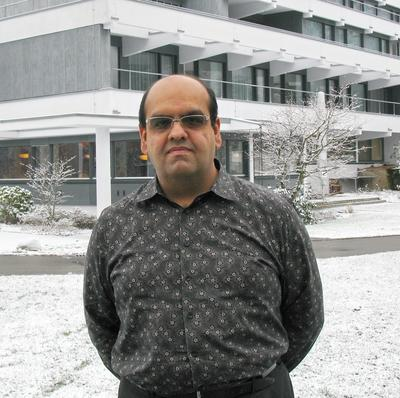
\includegraphics[height=0.42\textheight]{ch2_cont_2012.jpg}\\[1mm]
\imgcap{Rama Cont}
\imgcredit{https://commons.wikimedia.org/wiki/File:Rama_Cont_Oberwolfach_2012.jpg}{Photo: Renate Schmid (2012); CC BY-SA 2.0 DE; Wikimedia Commons}
\end{column}
\end{columns}
\end{frame}

\begin{frame}{Six Stylised Facts}
\itemsize{\small}
\begin{itemize}
    \item \textbf{1. Heavy tails}: large moves are far more frequent than under the Normal distribution
    \item \textbf{2. Aggregational Gaussianity}: returns over longer horizons are closer to the Normal distribution
    \item \textbf{3. Absence of linear autocorrelation}: past returns barely predict future returns
    \item \textbf{4. Volatility clustering}: large moves follow large moves, of either sign
    \item \textbf{5. Leverage effect}: falls raise future volatility more than rises
    \item \textbf{6. Gain/loss asymmetry}: large losses are larger and more frequent than large gains
\end{itemize}
\end{frame}

\begin{frame}{Fact 1: Heavy Tails, Counted}
\itemsize{\footnotesize}
\begin{center}
\footnotesize
\begin{tabular}{lrrrrrr}
\toprule
Series & $n$ & $>3\sigma$ & $>4\sigma$ & $>5\sigma$ & $>6\sigma$ & p-value (Poisson, $4\sigma$) \\
\midrule
S\&P 500 & 4\,201 & 62 & 28 & 12 & 8 & ${2 \times 10^{-46}}$ \\
DAX & 4\,244 & 56 & 20 & 5 & 4 & ${1 \times 10^{-30}}$ \\
BET & 4\,186 & 70 & 28 & 16 & 11 & ${2 \times 10^{-46}}$ \\
Bitcoin & 4\,384 & 80 & 29 & 10 & 4 & ${6 \times 10^{-48}}$ \\
Normal distribution, $n = 4\,201$ & & $11.34$ & $0.27$ & $2.4 \times 10^{-3}$ & $8.3 \times 10^{-6}$ &  \\
\bottomrule
\end{tabular}
\end{center}
\begin{itemize}
    \item $>k\sigma$: number of days with $|r_t - \bar r| > k\,s$; last row: number expected under the Normal distribution
    \item p-value: probability of at least that many 4-sigma days if the Normal count is Poisson with mean $n \times 6.3 \times 10^{-5}$
    \item S\&P 500: 105 times more 4-sigma days than the Normal distribution allows
\end{itemize}\sfmquantlet{Ch_02}{SFM_ch2_sigma_days}
\end{frame}

\begin{frame}{Fact 1: 4-Sigma Days in Every Market}
\itemsize{\footnotesize}
\begin{center}
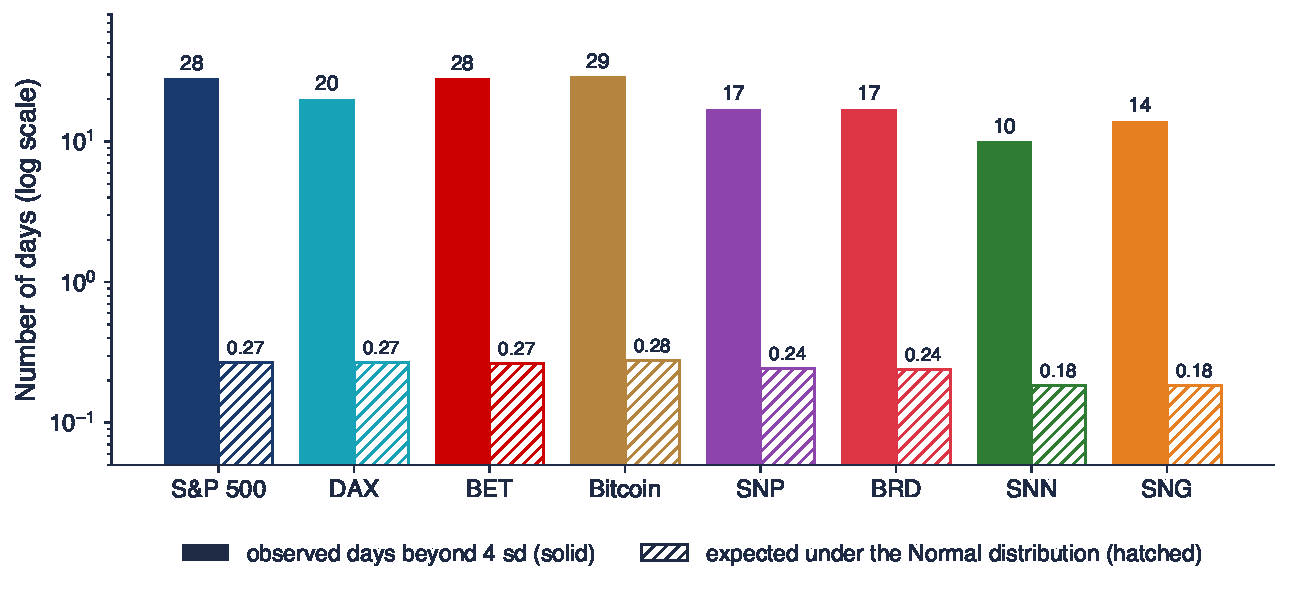
\includegraphics[width=0.97\textwidth,height=0.60\textheight,keepaspectratio]{sfm_ch2_sigma_days.pdf}
\end{center}
\vspace{-0.25cm}
\begin{itemize}
    \item Observed days beyond 4 standard deviations (log scale) against the Normal expectation of $0.18$--$0.28$ days
    \item Indices and Bitcoin: one 4-sigma day every 150--212 days; BVB stocks: 10--17 days in total
    \item Under a fitted Student-$t$, the expected numbers are close to the observed ones: S\&P 500 34.9, BET 28.1 (Seminar 2, B4)
\end{itemize}
\sfmquantlet{Ch_02}{SFM_ch2_sigma_days}
\end{frame}

\begin{frame}{Fact 2: Aggregational Gaussianity}
\itemsize{\small}
\begin{itemize}
    \item $h$-day log return: $r_t(h) = r_t + r_{t-1} + \dots + r_{t-h+1}$, taken on non-overlapping blocks
    \begin{itemize}
        \item if the CLT applies, the distribution of $r_t(h)$ approaches the Normal distribution as $h$ grows
    \end{itemize}
    \item The stylised fact: the shape changes with the horizon; it is not the same at all time scales \refCont
    \item Price to pay: fewer observations
    \begin{itemize}
        \item S\&P 500, 17 years: 4\,201 daily, 200 monthly and 66 quarterly returns
        \item estimates of kurtosis at long horizons are very noisy
    \end{itemize}
\end{itemize}
\end{frame}

\begin{frame}{Fact 2: Kurtosis Falls with the Horizon}
\itemsize{\footnotesize}
\begin{center}
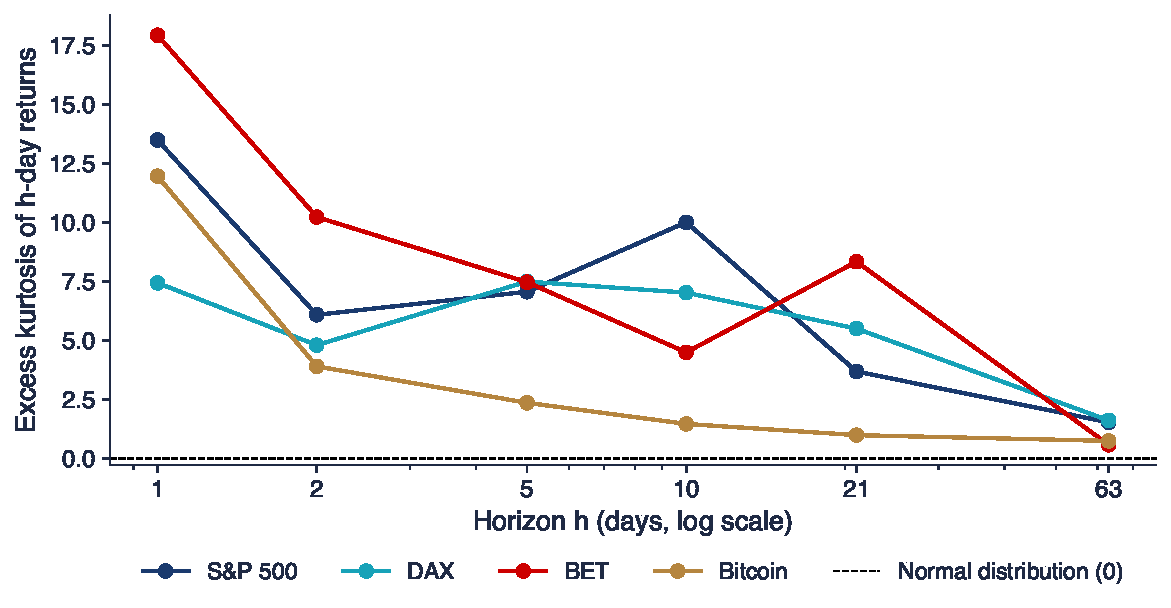
\includegraphics[width=0.97\textwidth,height=0.60\textheight,keepaspectratio]{sfm_ch2_aggregation.pdf}
\end{center}
\vspace{-0.25cm}
\begin{itemize}
    \item Excess kurtosis, daily $\to$ monthly $\to$ quarterly: S\&P 500 13.5 $\to$ 3.7 $\to$ 1.5; BET 17.9 $\to$ 8.3 $\to$ 0.6; Bitcoin 12.0 $\to$ 1.0 $\to$ 0.7
    \item The fall is slow and not monotone: one crash month (March 2020) dominates a sample of 200 months
    \item Quarterly returns: JB no longer rejects normality for the BET (p-value $0.07$) and Bitcoin (p-value $0.22$)
\end{itemize}
\sfmquantlet{Ch_02}{SFM_ch2_cont_stylised_facts}
\end{frame}

\begin{frame}{Fact 2: S\&P 500, Daily vs Monthly QQ Plots}
\itemsize{\footnotesize}
\begin{center}
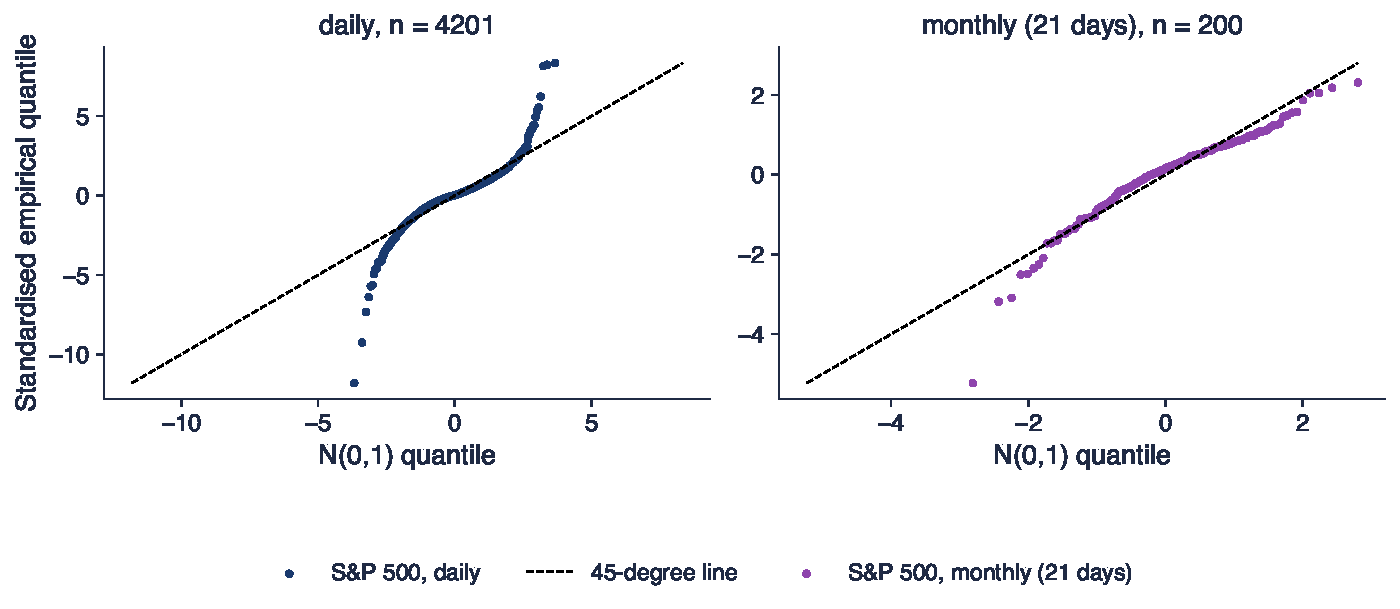
\includegraphics[width=0.97\textwidth,height=0.60\textheight,keepaspectratio]{sfm_ch2_qq_horizons.pdf}
\end{center}
\vspace{-0.25cm}
\begin{itemize}
    \item Monthly returns lie much closer to the line than daily returns
    \item But monthly returns are not Normal: skewness $-1.18$, excess kurtosis $3.7$, $n = 200$; the lowest point is March 2020
    \item Why so slow? Volatility clustering makes daily returns dependent, which slows the CLT
\end{itemize}
\sfmquantlet{Ch_02}{SFM_ch2_cont_stylised_facts}
\end{frame}

\begin{frame}{Fact 3: Absence of Linear Autocorrelation}
\itemsize{\small}
\begin{itemize}
    \item \textbf{ACF} (autocorrelation function): $\rho(h) = \text{Corr}(r_t, r_{t-h})$, $h = 1, 2, \dots$
    \begin{itemize}
        \item sample version $\hat\rho(h) = \sum_t (r_t - \bar r)(r_{t-h} - \bar r)/\sum_t (r_t - \bar r)^2$
        \item $h$: the lag in days; $\rho(h) \in [-1, 1]$; for i.i.d. data, $\hat\rho(h) \approx N(0, 1/n)$: 95\% band $\pm 1.96/\sqrt{n}$
    \end{itemize}
    \item \textbf{LB} (Ljung--Box) test \refLB{} of $H_0$: $\rho(1) = \dots = \rho(m) = 0$
    \begin{itemize}
        \item $Q(m) = n(n+2)\sum_{h=1}^m \hat\rho(h)^2/(n - h) \sim \chi^2(m)$; for $m = 10$, reject if $Q > 18.3$
        \item $m$: the number of lags tested together; $Q$ adds up the squared autocorrelations, so large values mean some $\rho(h) \neq 0$
    \end{itemize}
    \item Why absent? If returns were predictable, traders would exploit it until the predictability disappears (efficient markets, \sfmchlink{https://danpele.github.io/SFM/EN/Courses/chapter7_efficient_markets_random_walk_vr.pdf}{Chapter 7})
\end{itemize}
\end{frame}

\begin{frame}{Facts 3 and 4: ACF of Returns and of Absolute Returns}
\itemsize{\footnotesize}
\begin{center}
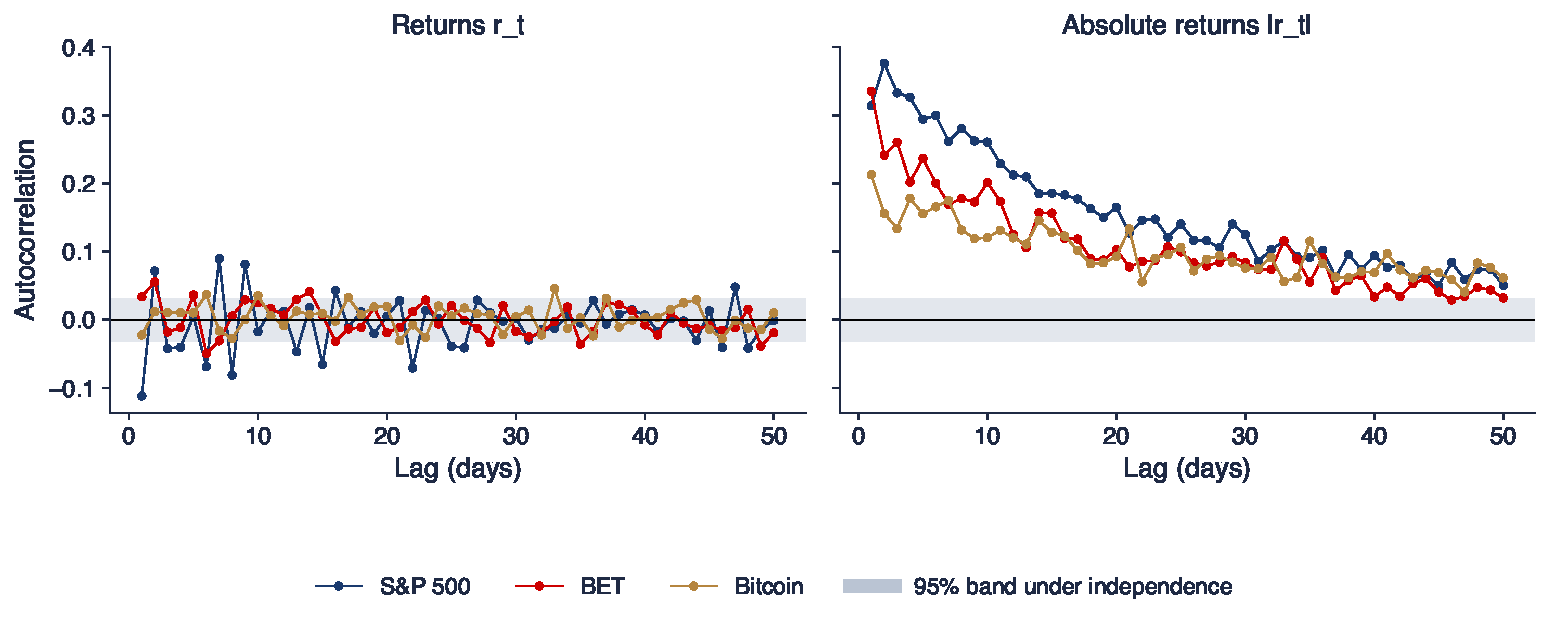
\includegraphics[width=0.97\textwidth,height=0.60\textheight,keepaspectratio]{sfm_ch2_acf.pdf}
\end{center}
\vspace{-0.25cm}
\begin{itemize}
    \item Left: returns; most autocorrelations are inside or close to the band; S\&P 500 $\hat\rho(1) = -0.11$, BET $0.03$, Bitcoin $-0.02$
    \item Right: absolute returns; all positive, slowly decaying: S\&P 500 $0.31$ at lag 1, $0.26$ at lag 10, $0.05$ at lag 50
\end{itemize}
\sfmquantlet{Ch_02}{SFM_ch2_cont_stylised_facts}
\end{frame}

\begin{frame}{Fact 3: Small but Not Always Zero}
\itemsize{\small}
\begin{itemize}
    \item Ljung--Box $Q(10)$ for returns: S\&P 500 199, BET 46, Bitcoin 20; critical value 18.3
    \begin{itemize}
        \item formally, some autocorrelation is significant
    \end{itemize}
    \item Two reasons not to over-read this
    \begin{itemize}
        \item the values are economically small: $|\hat\rho(h)| \le 0.11$, so at most 1.2\% of the variance is explained
        \item the band $\pm 1.96/\sqrt{n}$ assumes i.i.d. returns; with volatility clustering it is too narrow, so ``significant'' is found too often
    \end{itemize}
    \item The S\&P 500 value at lag 1 comes mostly from March 2020, when large falls and rebounds alternated: without 20 February--30 April 2020, $\hat\rho(1) = -0.04$
    \item Robust tests of predictability (variance ratios): \sfmchlink{https://danpele.github.io/SFM/EN/Courses/chapter7_efficient_markets_random_walk_vr.pdf}{Chapter 7}
\end{itemize}
\end{frame}

\begin{frame}{Fact 4: Volatility Clustering}
\itemsize{\footnotesize}
\begin{columns}[T]
\begin{column}{0.62\textwidth}
\begin{itemize}
    \item ``Large changes tend to be followed by large changes, of either sign, and small changes tend to be followed by small changes'' \refMandelbrot
    \item The sign of tomorrow's return is unpredictable; its size is not
    \item Evidence: ACF of $|r_t|$ positive for 50 lags
    \begin{itemize}
        \item Ljung--Box $Q(10)$ of $|r_t|$: S\&P 500 3859, BET 2120, Bitcoin 1086
    \end{itemize}
    \item So returns are uncorrelated but \textbf{not independent}
    \item Models: ARCH and GARCH (\sfmchlink{https://danpele.github.io/SFM/EN/Courses/chapter9_arch_garch_models.pdf}{Chapter 9})
\end{itemize}
\end{column}
\begin{column}{0.34\textwidth}
\centering
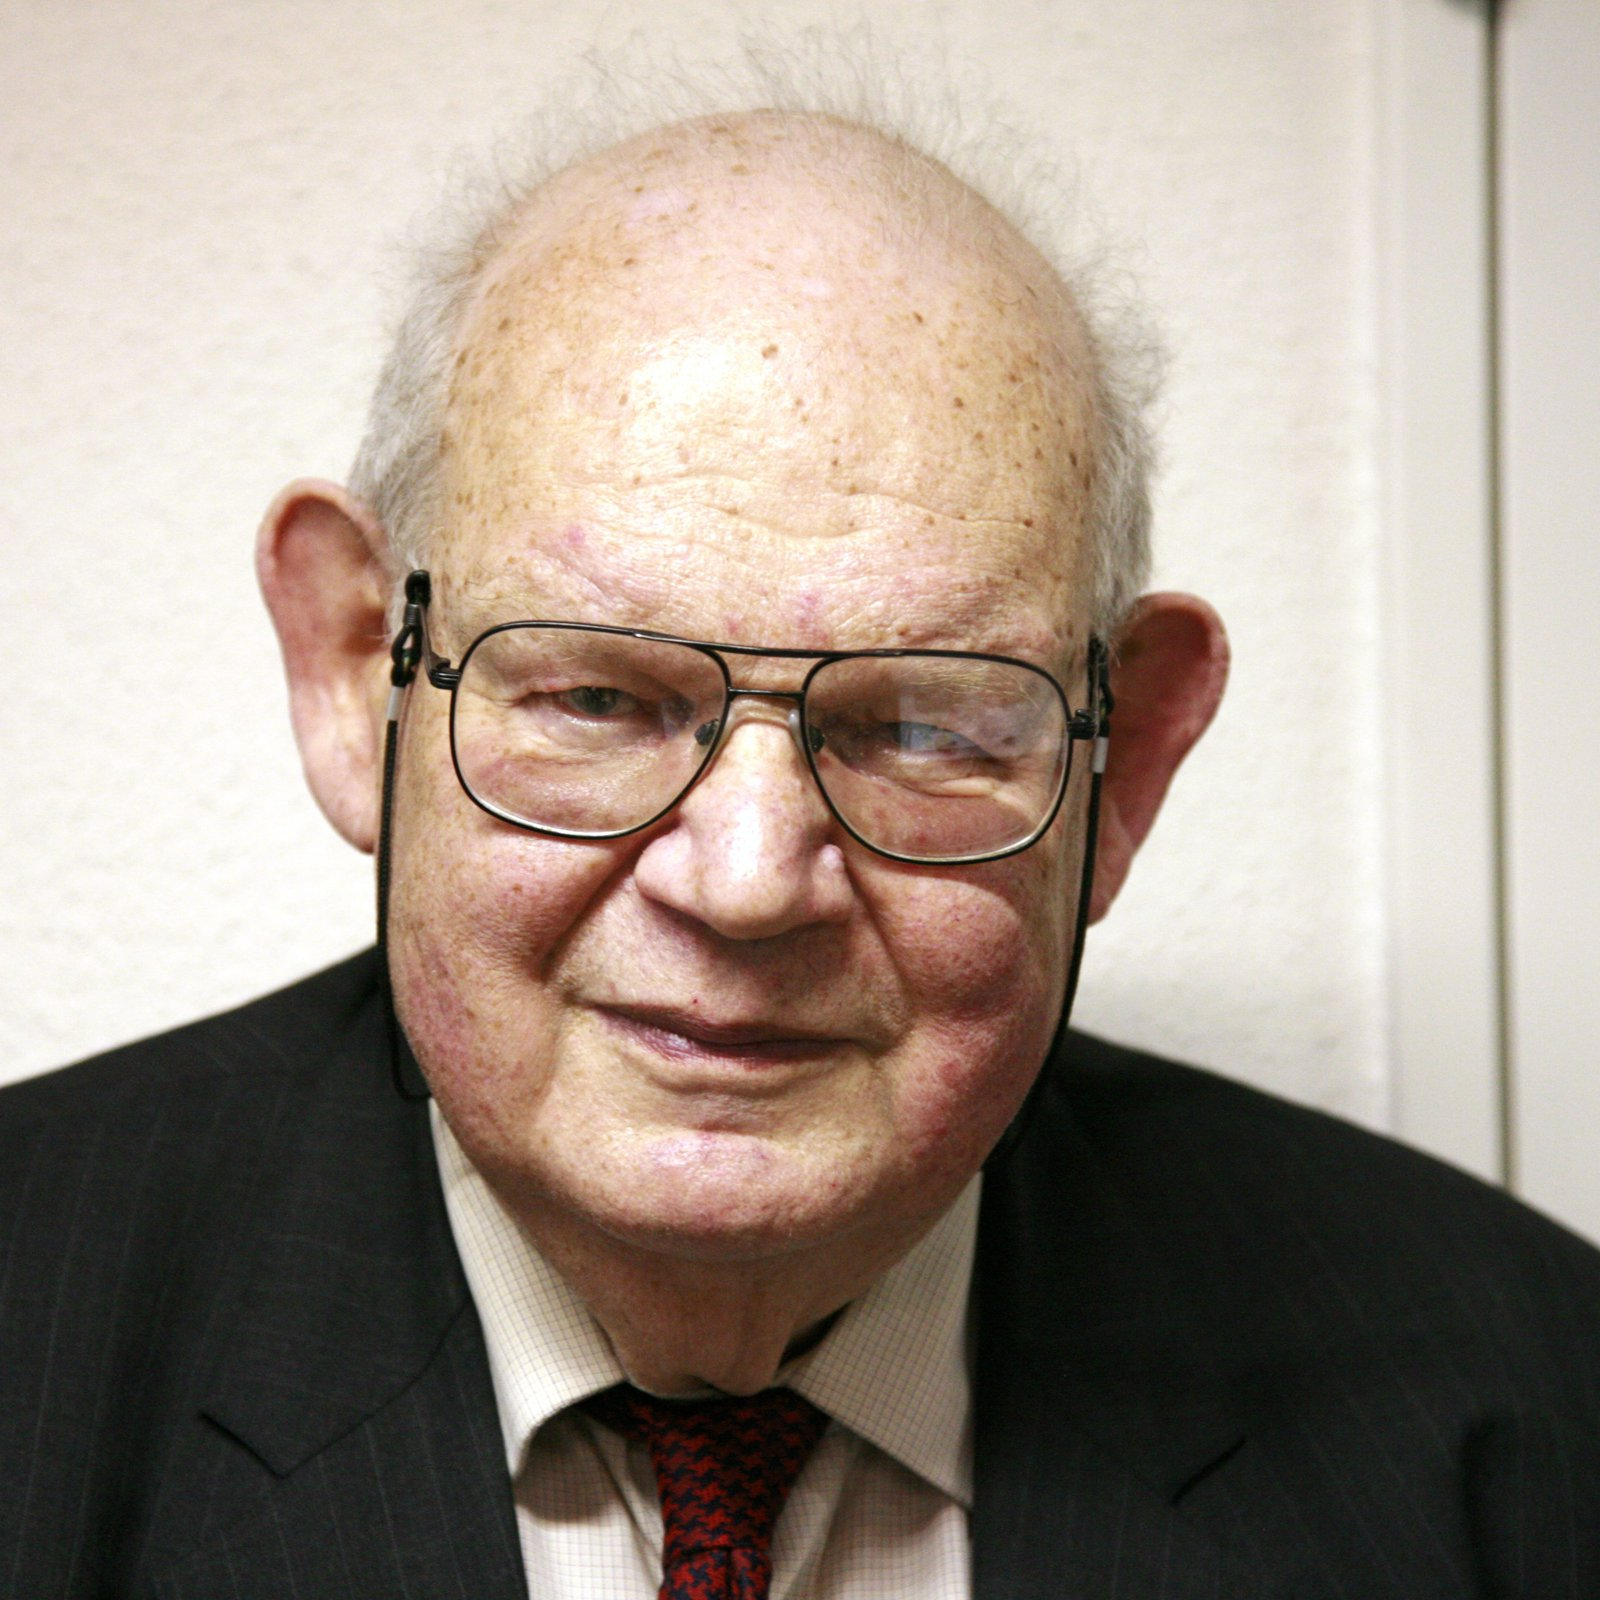
\includegraphics[height=0.42\textheight]{ch0_mandelbrot_2007.jpg}\\[1mm]
\imgcap{Benoit Mandelbrot (1924--2010)}
\imgcredit{https://commons.wikimedia.org/wiki/File:Benoit_Mandelbrot_mg_1804-d.jpg}{Photo: Rama (2007); CC BY-SA 2.0 fr; Wikimedia Commons}
\end{column}
\end{columns}
\end{frame}

\begin{frame}{Fact 4: Calm and Turbulent Periods}
\itemsize{\footnotesize}
\begin{center}
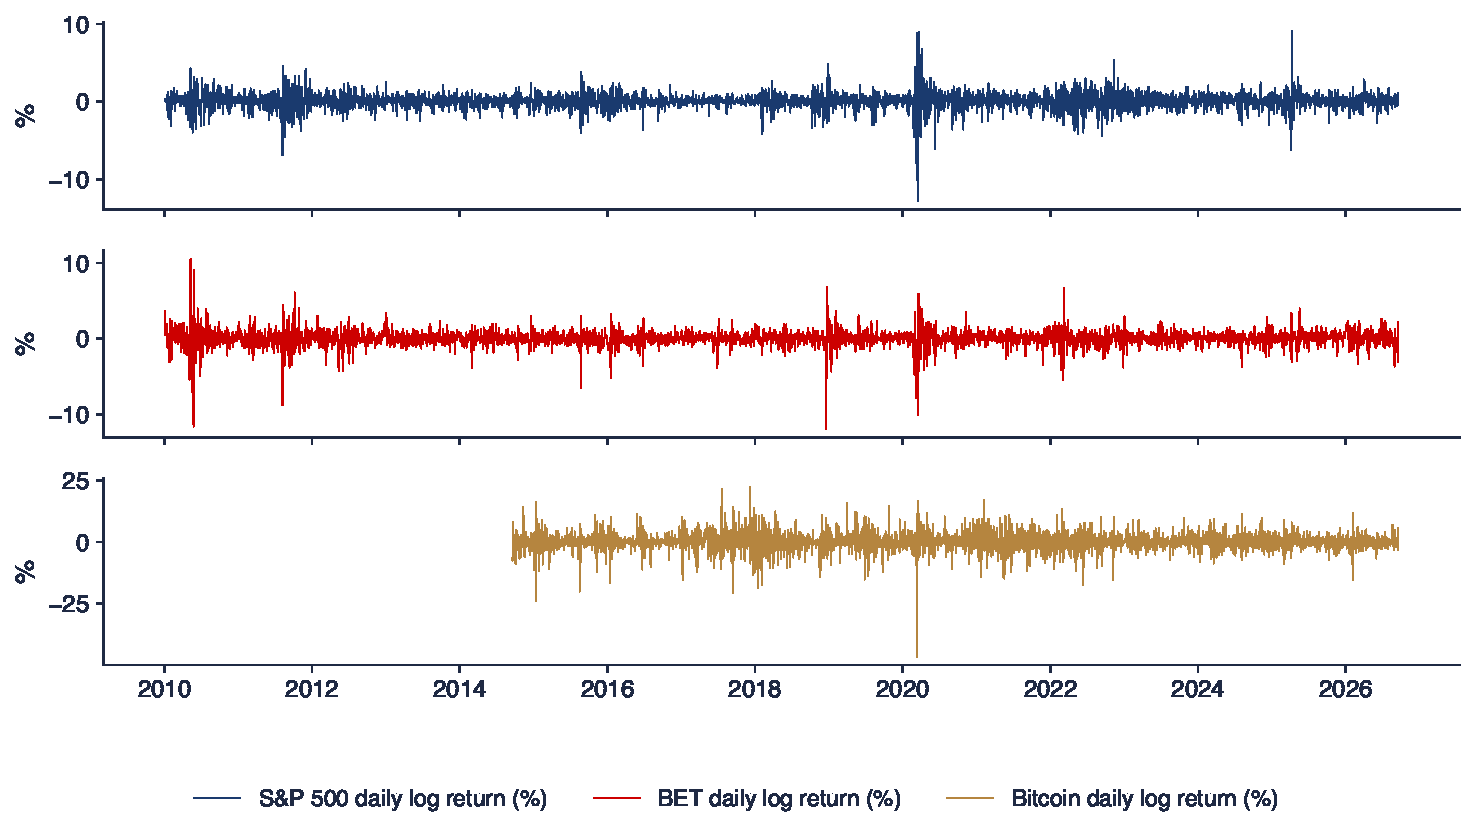
\includegraphics[width=0.97\textwidth,height=0.62\textheight,keepaspectratio]{sfm_ch2_clustering.pdf}
\end{center}
\vspace{-0.25cm}
\begin{itemize}
    \item Turbulent periods: 2010--2011 (euro area debt crisis), December 2018 for the BET, March 2020 everywhere, April 2025
    \item Calm years in between: the volatility of a single day depends on the period it falls in
\end{itemize}
\sfmquantlet{Ch_02}{SFM_ch2_cont_stylised_facts}
\end{frame}

\begin{frame}{Fact 5: The Leverage Effect}
\itemsize{\small}
\begin{itemize}
    \item Measure: $L(k) = \text{Corr}(r_t, |r_{t+k}|)$, $k = 1, 2, \dots$
    \begin{itemize}
        \item $L(k) < 0$: a fall today is followed by larger moves than a rise of the same size
    \end{itemize}
    \item Explanation by financial leverage \refChristie
    \begin{itemize}
        \item when the share price falls, the debt-to-equity ratio rises, so equity becomes riskier
    \end{itemize}
    \item A second explanation, volatility feedback: higher expected volatility raises required returns and lowers prices
    \item Models with an asymmetric response (EGARCH, GJR-GARCH): \sfmchlink{https://danpele.github.io/SFM/EN/Courses/chapter9_arch_garch_models.pdf}{Chapter 9}
\end{itemize}
\end{frame}

\begin{frame}{Fact 5: Leverage Correlations}
\itemsize{\footnotesize}
\begin{center}
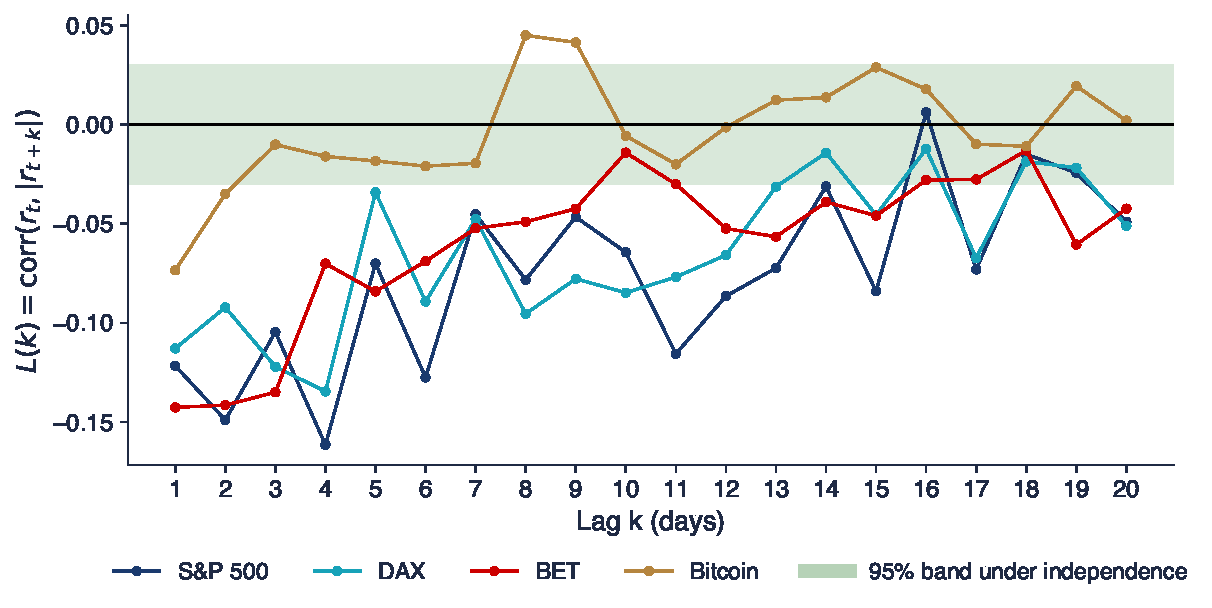
\includegraphics[width=0.97\textwidth,height=0.60\textheight,keepaspectratio]{sfm_ch2_leverage.pdf}
\end{center}
\vspace{-0.25cm}
\begin{itemize}
    \item Stock indices: $L(k) < 0$ for most of the first 20 lags; mean of $L(1..5)$: S\&P 500 $-0.12$, DAX $-0.10$, BET $-0.11$
    \item Bitcoin: $L(1) = -0.07$, then inside the band: no firm has debt behind Bitcoin, so the leverage mechanism is absent
\end{itemize}
\sfmquantlet{Ch_02}{SFM_ch2_cont_stylised_facts}
\end{frame}

\begin{frame}{Fact 6: Gain/Loss Asymmetry}
\itemsize{\footnotesize}
\begin{center}
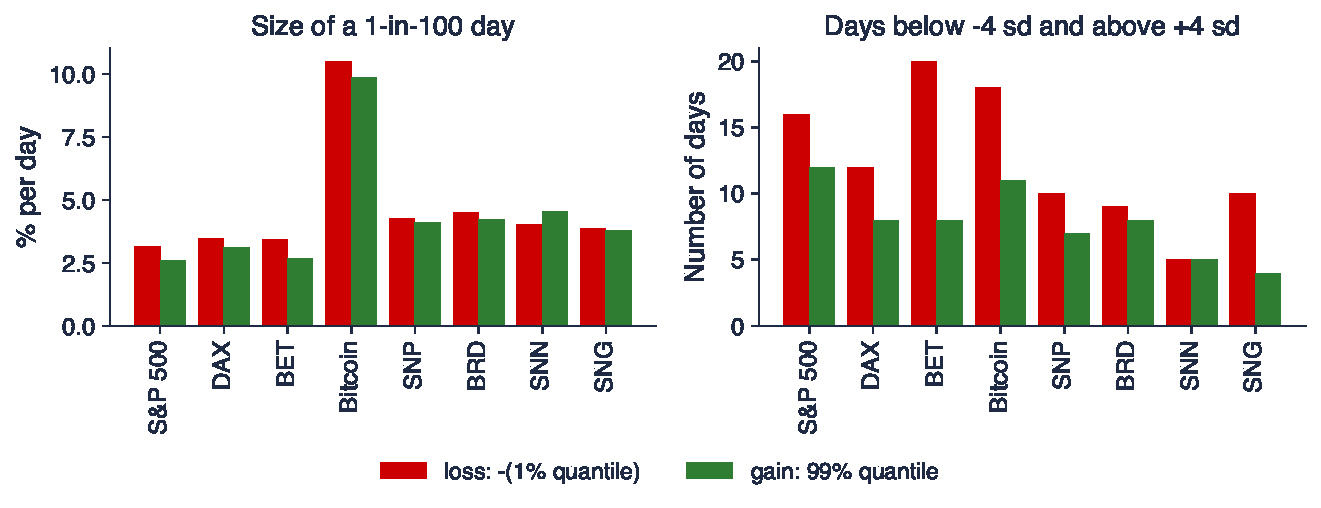
\includegraphics[width=0.97\textwidth,height=0.60\textheight,keepaspectratio]{sfm_ch2_gain_loss.pdf}
\end{center}
\vspace{-0.25cm}
\begin{itemize}
    \item Left: a 1-in-100 loss is larger than a 1-in-100 gain for the indices: BET 3.45\% vs 2.66\%, S\&P 500 3.15\% vs 2.61\%
    \item Right: days below $-4\sigma$ vs above $+4\sigma$: BET 20 vs 8, S\&P 500 16 vs 12, Bitcoin 18 vs 11
    \item Exception: SNN, with positive skewness and a larger right quantile
\end{itemize}
\sfmquantlet{Ch_02}{SFM_ch2_sigma_days}
\end{frame}

\begin{frame}{Six Facts, Eight Series}
\itemsize{\footnotesize}
\begin{center}
\scriptsize
\begin{tabular}{lrrrrrr}
\toprule
Series & Exc. kurt. & Exc. kurt., 21 days & $\hat\rho_r(1)$ & $\hat\rho_{|r|}(10)$ & $\bar L(1..5)$ & $|q_{0.01}|/q_{0.99}$ \\
\midrule
S\&P 500 & $13.5$ & $3.7$ & $-0.11$ & $0.26$ & $-0.12$ & $1.21$ \\
DAX & $7.4$ & $5.5$ & $0.01$ & $0.16$ & $-0.10$ & $1.12$ \\
BET & $17.9$ & $8.3$ & $0.03$ & $0.20$ & $-0.11$ & $1.30$ \\
Bitcoin & $12.0$ & $1.0$ & $-0.02$ & $0.12$ & $-0.03$ & $1.07$ \\
OMV Petrom (SNP) & $8.9$ & $3.3$ & $-0.02$ & $0.13$ & $-0.03$ & $1.04$ \\
BRD & $7.3$ & $0.4$ & $0.03$ & $0.11$ & $-0.05$ & $1.07$ \\
Nuclearelectrica (SNN) & $5.1$ & $2.3$ & $0.09$ & $0.08$ & $-0.03$ & $0.88$ \\
Romgaz (SNG) & $5.3$ & $1.4$ & $0.07$ & $0.08$ & $-0.04$ & $1.02$ \\
\bottomrule
\end{tabular}
\end{center}
\begin{itemize}
    \item Columns: excess kurtosis of daily and 21-day returns; ACF of returns at lag 1 and of $|r_t|$ at lag 10; mean $L(k)$ over lags 1--5; 1\% over 99\% quantile
    \item Facts 1, 3 and 4 hold for every series; fact 2 holds with noise; facts 5 and 6 hold for the indices and most BVB stocks, weakly or not for Bitcoin and SNN
    \item A comparison of the return distributions of cryptocurrencies and traditional assets: \refPeleCrypto
\end{itemize}\sfmquantlet{Ch_02}{SFM_ch2_cont_stylised_facts}
\end{frame}

\begin{frame}{What the Facts Mean for Models}
\itemsize{\small}
\begin{center}
\footnotesize
\begin{tabular}{lcccccc}
\toprule
Model & 1 & 2 & 3 & 4 & 5 & 6 \\
\midrule
i.i.d. Normal & -- & trivially & \checkmark & -- & -- & -- \\
i.i.d. Student-$t$ & \checkmark & \checkmark & \checkmark & -- & -- & -- \\
GARCH with $t$ errors (Ch.~9) & \checkmark & \checkmark & \checkmark & \checkmark & -- & -- \\
EGARCH, GJR-GARCH (Ch.~9) & \checkmark & \checkmark & \checkmark & \checkmark & \checkmark & (\checkmark) \\
\bottomrule
\end{tabular}
\end{center}
\begin{itemize}
    \item Columns: the six facts in the order of this section; (\checkmark): only for returns over several days, unless the errors are skewed
    \item Risk measures (VaR 1\%, ES 2.5\%, \sfmchlink{https://danpele.github.io/SFM/EN/Courses/chapter10_var_es_backtesting.pdf}{Chapter 10}) inherit the quality of the model: a Normal VaR is too low in crises
    \item A related summary of tail risk, information entropy: \refPeleEntropy
\end{itemize}
\end{frame}

\begin{frame}{Recap: Stylised Facts}
\itemsize{\small}
\begin{itemize}
    \item Heavy tails: 4-sigma days every few months instead of once in decades
    \item Returns are nearly uncorrelated, but their size is strongly autocorrelated
    \item Longer horizons are closer to the Normal distribution, slowly
    \item Stock indices: falls raise volatility, and losses are larger than gains
\end{itemize}
\end{frame}


%=============================================================================
\section{AI for Scientific Discovery}
%=============================================================================

\begin{frame}{An Open Question: Are Bitcoin's Tails Getting Thinner?}
\itemsize{\footnotesize}
\begin{columns}[T]
\begin{column}{0.50\textwidth}
\begin{center}
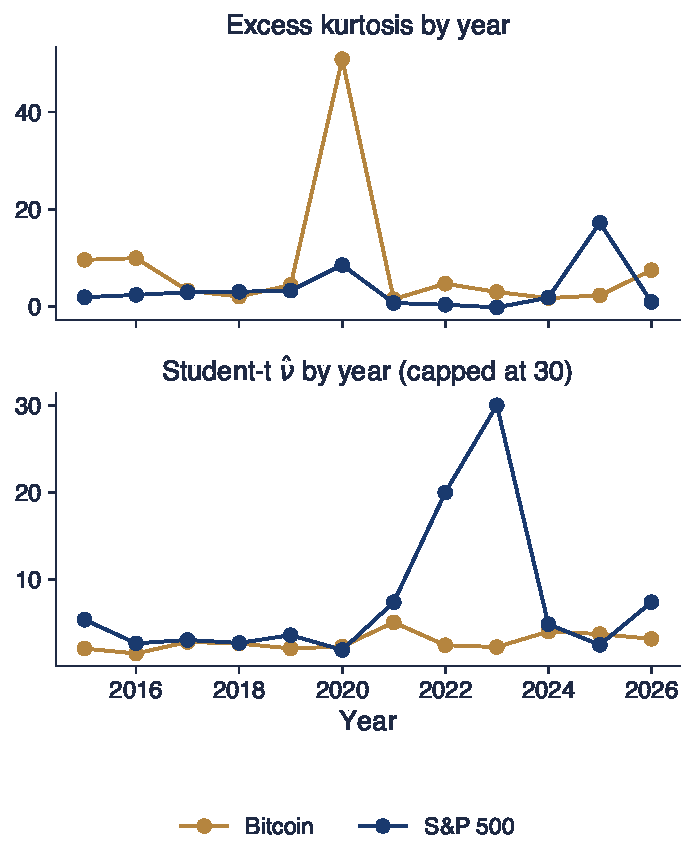
\includegraphics[width=\linewidth,height=0.72\textheight,keepaspectratio]{sfm_ch2_tails_by_year.pdf}
\end{center}
\end{column}
\begin{column}{0.46\textwidth}
\begin{itemize}
    \item As a market matures (more traders, futures, ETFs), its tails might thin out
    \item Bitcoin, 2015--2026: yearly $\hat\nu$ between 1.5 and 5.1; rank correlation with the year $0.63$ (p-value $0.03$)
    \item Why it is open: 12 noisy yearly estimates, one year (2020, excess kurtosis 51) dominated by one day
    \item AI tools can speed up such a study; they do not replace checking it \refWang
\end{itemize}
\end{column}
\end{columns}
\sfmquantlet{Ch_02}{SFM_ch2_tails_by_year}
\end{frame}

\begin{frame}{How AI Could Help}
\itemsize{\small}
\begin{itemize}
    \item \textbf{Literature}: find studies of tail indices of crypto assets and summarise their methods
    \item \textbf{Code}: draft rolling-window estimates of $\nu$ and of the excess kurtosis
    \item \textbf{Robustness}: propose other windows, other tail measures (\sfmchlink{https://danpele.github.io/SFM/EN/Courses/chapter5_heavy_tails_evt.pdf}{Chapter 5}), other crypto assets
    \item Example prompt
    \begin{itemize}
        \item \aiprompt{Write a Python function that fits a Student-t distribution to daily Bitcoin log returns on rolling 365-day windows and returns the degrees of freedom with a bootstrap 95\% interval.}
    \end{itemize}
\end{itemize}
\end{frame}

\begin{frame}{What to Check}
\itemsize{\small}
\begin{itemize}
    \item Data: the same price column and calendar for every year; errors among the largest moves
    \item Estimation: did the optimiser converge? $\hat\nu$ near 2 or above 30 needs a second look
    \item Inference: one $\hat\nu$ per year is noisy; report intervals, not only point estimates
    \item Volatility clustering: thinner yearly tails may only mean calmer years (\sfmchlink{https://danpele.github.io/SFM/EN/Courses/chapter9_arch_garch_models.pdf}{Chapter 9})
    \item References: every cited paper must exist; check the DOI
\end{itemize}
\end{frame}

\begin{frame}{Project Seed}
\itemsize{\small}
\begin{itemize}
    \item \textbf{Question}: do the tails of crypto assets thin out as their markets mature?
    \begin{itemize}
        \item data: Bitcoin, Ethereum and Solana from the course data; S\&P 500 as a benchmark
    \end{itemize}
    \item Steps
    \begin{itemize}
        \item estimate $\hat\nu$ and the excess kurtosis on rolling one-year windows, with bootstrap intervals
        \item test for a trend; repeat on returns divided by a rolling volatility
        \item compare the count of 4-sigma days per year with the S\&P 500
    \end{itemize}
    \item Deliverable: one table, one chart, and a paragraph on what the data can and cannot show
    \item Declare any AI use, and list the errors of the AI that you corrected
\end{itemize}
\end{frame}


%=============================================================================
\section{Summary}
%=============================================================================

\begin{frame}{Key Formulas}
\itemsize{\small}
\begin{center}
\footnotesize
\begin{tabular}{ll}
\toprule
\textbf{Quantity} & \textbf{Formula} \\
\midrule
Normal PDF & $f(x) = (\sigma\sqrt{2\pi})^{-1}\exp\big(-(x - \mu)^2/(2\sigma^2)\big)$ \\
Lognormal moments & median $e^m$, mean $e^{m + s^2/2}$ \\
CLT & $\sqrt{n}(\bar X_n - \mu)/\sigma \xrightarrow{d} N(0,1)$ \\
Skewness, excess kurtosis & $S = m_3/m_2^{3/2}$, \quad $K = m_4/m_2^2 - 3$ \\
Jarque--Bera & $\text{JB} = \frac{n}{6}(S^2 + K^2/4) \sim \chi^2(2)$ \\
Student-$t(\nu)$ & variance $\nu/(\nu - 2)$, excess kurtosis $6/(\nu - 4)$ \\
AIC & $2k - 2\ell$ \\
ACF, Ljung--Box & $\hat\rho(h)$, \quad $Q(m) = n(n+2)\sum_{h=1}^m \hat\rho(h)^2/(n - h)$ \\
Leverage & $L(k) = \text{Corr}(r_t, |r_{t+k}|)$ \\
\bottomrule
\end{tabular}
\end{center}
\end{frame}

\begin{frame}{Check Yourself}
\itemsize{\small}
\begin{itemize}
    \item \textbf{Question}: daily returns are $N(0.05\%, 1\%^2)$; how many standard deviations is a $-3\%$ day?
    \begin{itemize}
        \item \textbf{Answer}: $z = (-3 - 0.05)/1 = -3.05$
    \end{itemize}
    \item \textbf{Question}: $n = 2500$, $S = -0.5$, $K = 6$; what is JB?
    \begin{itemize}
        \item \textbf{Answer}: $\frac{2500}{6}(0.25 + 9) = 3854$; normality is rejected
    \end{itemize}
    \item \textbf{Question}: an annual log return is $N(5\%, 20\%^2)$; what are the median and the mean of 100 invested after one year?
    \begin{itemize}
        \item \textbf{Answer}: median $100e^{0.05} = 105.1$, mean $100e^{0.05 + 0.02} = 107.3$
    \end{itemize}
    \item Next: \sfmchlink{https://danpele.github.io/SFM/EN/Courses/chapter3_alpha_stable_distributions.pdf}{Chapter 3}, $\alpha$-stable distributions
\end{itemize}
\end{frame}


%=============================================================================
\section{References}
%=============================================================================

\begin{frame}{References (1/2)}
\itemsize{\tiny}
\begin{itemize}
    \item Akaike, H. (1974). \href{https://doi.org/10.1109/TAC.1974.1100705}{A new look at the statistical model identification}. \textit{IEEE Transactions on Automatic Control}, 19(6), 716--723.
    \item Bachelier, L. (1900). \href{https://doi.org/10.24033/asens.476}{Théorie de la spéculation}. \textit{Annales scientifiques de l'École Normale Supérieure}, 17, 21--86.
    \item Blattberg, R.C., Gonedes, N.J. (1974). \href{https://doi.org/10.1086/295634}{A comparison of the stable and Student distributions as statistical models for stock prices}. \textit{Journal of Business}, 47(2), 244--280.
    \item Bollerslev, T. (1987). \href{https://doi.org/10.2307/1925546}{A conditionally heteroskedastic time series model for speculative prices and rates of return}. \textit{Review of Economics and Statistics}, 69(3), 542--547.
    \item Borak, S., Härdle, W.K., López-Cabrera, B. (2013). \href{https://doi.org/10.1007/978-3-642-33929-5}{\textit{Statistics of Financial Markets: Exercises and Solutions}}, 2nd ed. Springer.
    \item Christie, A.A. (1982). \href{https://doi.org/10.1016/0304-405X(82)90018-6}{The stochastic behavior of common stock variances: value, leverage and interest rate effects}. \textit{Journal of Financial Economics}, 10(4), 407--432.
    \item Cont, R. (2001). \href{https://doi.org/10.1080/713665670}{Empirical properties of asset returns: stylized facts and statistical issues}. \textit{Quantitative Finance}, 1(2), 223--236.
    \item Fama, E.F. (1965). \href{https://doi.org/10.1086/294743}{The behavior of stock-market prices}. \textit{Journal of Business}, 38(1), 34--105.
    \item Franke, J., Härdle, W.K., Hafner, C.M. (2019). \href{https://doi.org/10.1007/978-3-030-13751-9}{\textit{Statistics of Financial Markets: An Introduction}}, 5th ed. Springer.
    \item Jarque, C.M., Bera, A.K. (1980). \href{https://doi.org/10.1016/0165-1765(80)90024-5}{Efficient tests for normality, homoscedasticity and serial independence of regression residuals}. \textit{Economics Letters}, 6(3), 255--259.
    \item Jarque, C.M., Bera, A.K. (1987). \href{https://doi.org/10.2307/1403192}{A test for normality of observations and regression residuals}. \textit{International Statistical Review}, 55(2), 163--172.
\end{itemize}
\end{frame}

\begin{frame}{References (2/2)}
\itemsize{\tiny}
\begin{itemize}
    \item Ljung, G.M., Box, G.E.P. (1978). \href{https://doi.org/10.1093/biomet/65.2.297}{On a measure of lack of fit in time series models}. \textit{Biometrika}, 65(2), 297--303.
    \item Mandelbrot, B. (1963). \href{https://doi.org/10.1086/294632}{The variation of certain speculative prices}. \textit{Journal of Business}, 36(4), 394--419.
    \item Osborne, M.F.M. (1959). \href{https://doi.org/10.1287/opre.7.2.145}{Brownian motion in the stock market}. \textit{Operations Research}, 7(2), 145--173.
    \item Pele, D.T., Lazar, E., Dufour, A. (2017). \href{https://doi.org/10.3390/e19050226}{Information entropy and measures of market risk}. \textit{Entropy}, 19(5), 226.
    \item Pele, D.T., Wesselhöfft, N., Härdle, W.K., Kolossiatis, M., Yatracos, Y.G. (2023). \href{https://doi.org/10.1080/1351847X.2021.1960403}{Are cryptos becoming alternative assets?} \textit{European Journal of Finance}, 29(10), 1064--1105.
    \item Praetz, P.D. (1972). \href{https://doi.org/10.1086/295425}{The distribution of share price changes}. \textit{Journal of Business}, 45(1), 49--55.
    \item Student (1908). \href{https://doi.org/10.1093/biomet/6.1.1}{The probable error of a mean}. \textit{Biometrika}, 6(1), 1--25.
    \item Tsay, R.S. (2010). \href{https://doi.org/10.1002/9780470644560}{\textit{Analysis of Financial Time Series}}, 3rd ed. Wiley.
    \item Wang, H., Fu, T., Du, Y., Gao, W., et al. (2023). \href{https://doi.org/10.1038/s41586-023-06221-2}{Scientific discovery in the age of artificial intelligence}. \textit{Nature}, 620, 47--60.
    \item Wilk, M.B., Gnanadesikan, R. (1968). \href{https://doi.org/10.1093/biomet/55.1.1}{Probability plotting methods for the analysis of data}. \textit{Biometrika}, 55(1), 1--17.
\end{itemize}
\end{frame}

\end{document}
